\documentclass[11pt]{article}
\usepackage{times}
\usepackage{amsmath,amsthm,amssymb,bbold, mathtools,setspace,enumitem,epsfig,titlesec,verbatim,color,array,multirow,comment,graphicx,hyperref,blkarray}
%\usepackage[sort&compress]{natbib} % ProcB
\usepackage[super,sort&compress,comma]{natbib} % NComms
\usepackage[bf,small]{caption}
\usepackage[export]{adjustbox}
\usepackage[top=2.5cm,left=2.8cm,right=2.8cm,bottom=3.2cm]{geometry} 
\smallskip 

\definecolor{darkred}{rgb}{0.6,0,0}
\definecolor{darkblue}{rgb}{0,0.3,0.8}

\newcommand{\christian}[1]{\textcolor{blue}{{\bf CH:} #1}} 

\titleformat{\section}{\sffamily \fontsize{12}{20}\bfseries}{\thesection}{1em}{}
\titleformat{\subsection}{\sffamily \fontsize{11}{20}\bfseries}{\thesubsection}{1em}{}

\renewcommand{\figurename}{Figure}


\newcommand{\FigIllustration}{{\bf Fig.~1}}

\newtheoremstyle{plainCl1}% name
{9pt}%      Space above, empty = 'usual value'
{15pt}%      Space below
{\it}% 	   Body font
{}%         Indent amount (empty = no indent, \parindent = para indent)
{\bfseries}% Thm head font
{.}%        Punctuation after thm head
{2mm}% Space after thm head: \newline = linebreak
{}%         Thm head spec

\newtheoremstyle{plainCl2}% name
{9pt}%      Space above, empty = 'usual value'
{15pt}%      Space below
{\it}% 	   Body font
{}%         Indent amount (empty = no indent, \parindent = para indent)
{\bfseries}% Thm head font
{.}%        Punctuation after thm head
{4mm}% Space after thm head: \newline = linebreak
{}%         Thm head spec

\theoremstyle{plainCl1}
\newtheorem{theorem}{Theorem}
\newtheorem{Prop}{Proposition}
\newtheorem{definition}{Definition}

\theoremstyle{plainCl2}
\newtheorem{lemma}{Lemma}
\newtheorem{proposition}{Proposition}
\newtheorem{Corollary}{Corollary}


\newcommand{\ALLD}{\emph{D}}

\newcommand{\A}{\mathbf{A}}
\newcommand{\abf}{\mathbf{a}}
\newcommand{\bbf}{\mathbf{b}}
\newcommand{\cbf}{\mathbf{c}}
\newcommand{\qbf}{\mathbf{q}}
\newcommand{\pbf}{\mathbf{p}}
\newcommand{\T}{\mathbf{T}}
\newcommand{\ubf}{\mathbf{u}}
\newcommand{\C}{\mathrm{C}}
\newcommand{\D}{\mathrm{D}}

%\title{\sffamily \Large Supplementary Information\\[0.1cm] {\bfseries Introspection dynamics in asymmetric multiplayers games}}
\title{\sffamily \Large {\bfseries Introspection dynamics in asymmetric multiplayers games}}
\date{\empty}
\author{\parbox[c]{16cm}{\centering \onehalfspacing \fontsize{11}{12}\selectfont Marta Couto$^{1*}$ and Saptarshi Pal$^{1*}$\\[0.2cm]
$^1$Max Planck Research Group Dynamics of Social Behavior, Max Planck Institute for Evolutionary Biology, 24306~Ploen, Germany}\\ \\
$^*$ \fontsize{11}{12}\selectfont co-first authors}



\begin{document}
\maketitle
\onehalfspacing
\section*{Abstract}

% 150 to 250 words
% 4 to 6 keywords: multiplayer games, asymmetric games, non-linear interactions, learning model, introspection dynamics, strategy abundance  

The simplest form of social interaction occurs between two nearly similar individuals. This scenario can be stylized in a pairwise symmetric game. 
More complex behavior emerges when instead we consider multiple interacting individuals, and they may differ significantly among themselves. This case can be captured by a multiplayer asymmetric game. The complexity of these games increases both with the number and diversity of players.
From evolutionary dynamics to learning models, game theoretic frameworks have been widely used to study strategic behavior. 
Introspection dynamics has proven to be a useful learning model for tackling complex games. 
It provides a simple way to compute the average abundance of each combination of strategies (or actions), that is, the stationary distribution of strategies.
Here, our aim is to analyse multiplayer and (a)symmetric games.
We extend previous analytical results on pairwise games under introspection dynamics to multiplayer games. 
For general games, we obtain the analytical stationary distribution for 2 strategies, symmetric games.
Moreover, we consider a particular class of games -- additive games. 
In additive games, for any player, the difference between the payoffs provided by any two actions is constant, regardless of the co-players' actions. 
For these games, we derive the stationary distribution analytically, for any number of players and strategies, with no restriction to symmetric games. 
To illustrate our theoretical results, we analyse various multiplayer asymmetric social dilemmas. 
In general, players that have a lower cost or a higher benefit of cooperation learn to cooperate more frequently.
% 244 words

%In addition, we find that the frequency of a state (a combination of actions played by each player) corresponds to the product of the frequencies of each player playing their respective strategy.


\begin{comment}
The simplest form of social interaction occurs between two nearly similar individuals. This scenario can be stylized in a pairwise symmetric game. 
More complex behavior emerges when instead we consider multiple interacting individuals, and they may differ significantly among themselves. This case, in turn, can be captured by a multiplayer asymmetric game. The complexity of these games increases both with the number and diversity of players.
From evolutionary dynamics to learning models, game theoretic frameworks have been widely used to study strategic behavior. 
Introspection dynamics has proven to be a useful learning model to tackle complex games.
%To analyse more complex games, researchers typically use approximations, e.g. weak selection, small mutation. 
Here, our aim is to analyse multiplayer and (a)symmetric games. We extend previous analytical results of pairwise games under introspection dynamics to multiplayer games. 
We divide games into two main categories: additive and non-additive (or general) games.
In additive games, for any player, the difference between the payoffs provided by any two actions (or strategies) is constant, regardless of the co-players' actions. 
Non-additive are all games that do not hold this property; hence, general games.
For additive games, we derive the stationary distribution of strategies analytically, for any number of players and strategies. 
%Additionally, we find that the joint distribution of strategies factorizes over the marginal distribution of strategies.
Additionally, we find that the frequency of a state (a combination of actions played by each player) corresponds to the product of the frequencies of each player playing their respective strategy.
For non-additive games, we obtain the analytical stationary distribution for 2-strategies symmetric games. For other cases, we provide numerical results. 
To illustrate our theoretical results, we analyse various multiplayer asymmetric social dilemmas. 
In general, players that have a lower cost or a higher benefit of cooperation learn to cooperate more frequently.
%add rewarding game
\end{comment}
\newpage

\section*{Introduction}

%[Multiplayer games]

% Pairwise vs Multiplayer Games
The simplest form of social interaction occurs between two individuals. These pairwise interactions have been studied extensively \cite{Hofbauer:book:1998}. Despite their simplicity, they provide important insights, e.g., on how social species can maintain cooperation \cite{Axelrod:book:1984, Nowak:book:2011}. An ubiquitous example of a model game for two players is the prisoner's dilemma. There, the two individuals have a temptation to cheat on each other, while both would be better off by offering mutual help. Solving this apparent paradox has been the focus of many studies, where various explanations were proposed \cite{Nowak:Science:2006}. 
%some references
\\ \\
% non-linearity
\noindent Yet, many interesting collective behaviors occur when multiple individuals interact simultaneously \cite{Palm:JMB:1984, Skyrms:book:2003, Pacheco:PRSB:2009, Archetti:EL:2011, Archetti:JTB:2012, Gokhale:DGAA:2014, Hilbe:JTB:2015, Venkateswaran:PRSB:2019}.
Importantly, most of these situations cannot be captured by the sum of several pairwise interactions. Thus, to account for such non-linearities, we need to consider multiplayer games \cite{Gokhale:DGAA:2014}. One well-known effect that only emerges when more than two players are present is the ``second-order free-riding problem" \cite{Fowler:PNAS:2005}. A natural solution to maintain pro-social behavior in a community is to monitor and punish defectors (and/or reward cooperators). However, most forms of sanctioning are considerably costly \cite{Henrich:Science:2006}. Therefore, an additional (second-order) dilemma is at stake: deterring defection is beneficial for all, but an individual that does not pay the associated cost has an advantage over the ones that do. As such, peer-punishment and sanctioning institutions can be hard to sustain without additional mechanisms or a suitable design \cite{Panchanathan:Nature:2004, Perc:SciRep:2012, Hilbe:SciRep:2012, Couto:JTB:2020, Pal:NatCom:2022}.
\\ \\
\noindent 
% size
Another interesting effect that multiplayer games allow exploring is that of the scale or size of the interaction itself. In situations that require some sort of coordination and where expectations on others play an important role in one's decisions (like in stag-hunt games), a growing group size might hinder the optimal outcome \cite{Skyrms:book:2003}. Likewise, it has been shown that it is hard to cooperate in large groups for some conditions \cite{Santos:PNAS:2011, Hilbe:JTB:2015}.
This is not a general effect, though. It can happen that adding more players actually promotes cooperation. Gokhale et al. \cite{gokhale:JTB:2011} investigate the 2-player and 3-player cases of a task allocation problem. Although the underlying rules defining the interactions are the same for the two cases, simply introducing a third player changes the overall game, resulting in a decrease in freeloading.
%As a biological example, consider a task allocation problem in a bacterial system. A strain of bacteria can do any of three actions: to specialize in producing one of two kinds of enzymes (at some personal cost) or not to produce any enzyme. The bacteria need two different types of enzymes at the same time to obtain resources from the environment. In \cite{gokhale:JTB:2011}, authors investigate both the 2-player and 3-player cases of this scenario. Although the underlying rules defining the interactions are the same for the two cases, simply introducing a third player changes the overall game, and hence the outcomes. With three players, the production of one of the enzymes increases while freeloading decreases, compared to the 2-player case.
Additionally, not only the average group size can have an important effect, but also the variance of the group size distribution \cite{Pena:Evolution:2011, Broom:BMB:2019}.
\\ \\ 
%[Asymmetric (multiplayer) games]
\noindent Complexity further increases when players differ significantly among themselves. This diversity can be captured by asymmetric games \cite{Taylor:JAP:1979, Schuster:AB:1981, Gaunersdorfer:TPB:1991, Hofbauer:JMB:1996, Hofbauer:GEB:2005, Ohtsuki:JTB:2010, McAvoy:PlosCB:2015, Veller:JET:2016, Hauser:Nature:2019}. In symmetric games, all players are indistinguishable. Thus, to fully characterise the state of the game, we only require to know the number of players playing each strategy. Conversely, in asymmetric games, players can be different in several ways. We say they are of different types or roles, which can differ in payoffs and strategies. Therefore, they can have uneven effects on others' payoffs too. For example, in public goods games and collective-risk dilemmas, players can have different initial endowments (or wealth), productivitites, costs, risk perceptions, or risk exposures \cite{Milinski:CC:2011, Vasconcelos:PNAS:2014, Abouchakra:JTB:2014, Hauser:Nature:2019, Merhej:JAIR:2022}. Hence, to fully describe the state of the game, we need to know which of the players is doing what. This greatly increases the size of the game's state space; even more so, for more than two players.  \\ \\ 
%meta communication; lit gap; our aim
\noindent From this, we see how the mathematical analysis of multiplayer asymmetric games can become cumbersome, the extreme cases being many-player games where all individuals are different. Perhaps for that reason, there are not many studies on a general approach to multiplayer asymmetric games. As such, our aim here is to narrow that gap using introspection dynamics \cite{Couto:NJP:2022}. In the following section, we discuss several canonical frameworks from the literature that have been used to study both multiplayer and asymmetric games.%, pointing out the gaps.

%possibly new section \section*{Background} but then where to put "proposal"?

\section*{Related Work}

%[Frameworks]

% deterministic EGT
From evolutionary game theory (EGT) \cite{Maynard-Smith:Nature:1973, Maynard-Smith:book:1982, Hofbauer:book:1998, Nowak:book:2006} to learning models \cite{Sandholm:BioSys:1996, Fudenberg:book:1998b, Macy:PNAS:2002, Pangallo:GEB:2022}, game theoretic frameworks have been widely used to study strategic behavior. 
In evolutionary game theory, we assume a population of players and a mechanism by which strategies evolve over time. More successful strategies tend to persist in the population, either by genetic or cultural inheritance. The first key concept in evolutionary game theory is ``evolutionary stable strategy" (ESS),  introduced in 1973, in the seminal paper of John Maynard Smith and George Price \cite{Maynard-Smith:Nature:1973}. A (monomorphic) population playing an ESS cannot be invaded by mutants. The concept of ESS, originally proposed for parwise encounters, was already extended for multiplayer games \cite{Palm:JMB:1984, Broom:BMB:1997, Bukowski:IJGT:2004}. Although suggestive of an evolutionary process, ESS does not really describe a dynamical system. In the more classical infinite population models (deterministic EGT), ordinary differential equations are the central mathematical tools \cite{Hofbauer:book:1998}. One of the most famous of these dynamics is the replicator equation \cite{Taylor:MB:1978, Hofbauer:book:1998}. Replicator equation has been widely used and easily comprises multiplayer games \cite{Hauert:JTB:2006a, gokhale:PNAS:2010, Pena:Evolution:2011, Cressman:PNAS:2014, Pena:JTB:2014}. More recently, also the replicator-mutator equation was applied to study the dynamics of multiplayer games \cite{Duong:DGAA:2020}. As for asymmetric games, a few additional assumptions are needed. For example, if there are two different types of players, typically, either there are two populations co-evolving (``bimatrix games" \cite{Hofbauer:book:1998, Gokhale:PRSB:2012, Tuyls:SciRep:2018}) or there is a single population of players where each can play the two types or roles (``role games") \cite{Hofbauer:book:1998}. For role games, a strategy must include the action played in each of the two roles. The case of asymmetric games with more than two players is substantially less studied within deterministic EGT. Exceptions are  \cite{Gokhale:PRSB:2012, Zhang:arxiv:2022}. Notably, although these works study multiplayer games, they consider, at most, two different types (drawn from two populations), which leaves out the exploration of full asymmetry.
% models of multiple populations seem unnatural
\\ \\
% stochastic EGT
\noindent To account for stochastic effects naturally present in finite populations, another set of tools was developed, known as stochastic evolutionary game dynamics.  \cite{Nowak:Nature:2004, Traulsen:bookchapter:2009}. Besides the finiteness of population sizes, it also considers random mutations. Here, the quantities of interest are fixation probabilities and fixation times (i.e., the probability and the average time that a single mutant overtakes an initially monomorphic population) for when mutations are rare \cite{Fudenberg:TPB:2006}, or average strategy abundance (i.e., the stationary distribution of strategy frequencies) for when mutation rates take intermediate values \cite{antal:JTB:2009a, antal:JTB:2009b}. 
\\ \\
%When deriving fixation probabilities and times, it is assumed that mutations are rare, such that, no new mutant arises between the very first and its eventual fixation \cite{}. 
%\cite{Chalub:BMB:2019}
\noindent 
These frameworks have been applied to asymmetric games assuming co-evolving (finite) subpopulations of different player types. Fixation probabilities for asymmetric 2-player \cite{Sekiguchi:DGA:2017}, asymmetric 3-player games \cite{Sekiguchi:DGAA:2022}, and symmetric multiplayer games \cite{Kurokawa:PRSB:2009, gokhale:PNAS:2010} were recently derived. Whereas with intermediate mutation, strategy abundances were obtained only for 2-player asymmetric games \cite{Ohtsuki:JTB:2010, Sekiguchi:PA:2013} or multiplayer symmetric games \cite{gokhale:JTB:2011, Wu:Games:2013}. For a review on evolutionary multiplayer games both in infinitely large populations as well as in finite populations, we refer to \cite{Gokhale:DGAA:2014}.\\ 
%comment on the pervasiveness of weak selection
%strategy abundance papers (intermediate mutation or mutation-selection equilibrium)
%2-player symmetric and asymmetric games, any number of strategies, Birth-death process \cite{ohtsuki:JTB:2010}
%2-player symmetric and asymmetric games, any number of strategies, Death-birth process \cite{Sekiguchi:PA:2013}

% multiplayer 
%\cite{gokhale:PNAS:2010}
%\cite{gokhale:JTB:2011} extends the approach in \cite{antal:JTB:2009b} for 2-player to multiplayer (symmetric) games. 
%\cite{Wu:Games:2013} symmetric, any number of strategies, Birth-death process (equations connections?)
%\cite{Gokhale:DGAA:2014} review on evolutionary multiplayer games both for infinitely large populations as well as finite population

% nice multiplayer applications

%[Learning models] IM NOT VERY HAPPY WITH HOW THIS SECTION READS YET
%learning models in general
\noindent Different from evolutionary game theory, learning models (of strategic behavior) take another approach \cite{Sandholm:BioSys:1996, Fudenberg:book:1998b, Macy:PNAS:2002, Hofbauer:GEB:2005, Tuyls:bookchapter:2005, Galla:PNAS:2013, Barfuss:PRE:2019, Barfuss:PNAS:2020, Pangallo:GEB:2022}. There is no evolution of strategies in a population necessarily, but a process by which individuals learn strategies dynamically. 
Despite the conceptual disparities, there have been already some efforts in unifying the two lines of research of evolutionary game theory and multiagent reinforcement learning \cite{Macy:PNAS:2002, Tuyls:bookchapter:2005, Bloembergen:JAIR:2015, Zhang:arxiv:2022}. 
\noindent Clearly, we can distinguish two different pathways that led to ``learning in games": one which stemmed from the broad field of reinforcement learning \cite{Sandholm:BioSys:1996} and the other from the classical game theory itself \cite{Fudenberg:book:1998b}. The ``theory of learning in games" was proposed as a refinement of classical equilibrium concepts, like Nash equilibrium, where strict assumptions of common knowledge of rationality are made. Instead, learning consists of ``\textit{an alternative explanation that equilibrium arises as the long-run outcome of a process in which less than fully rational players grope for optimality over time}" \cite{Fudenberg:book:1998b}. In this context, several learning models were introduced, such as fictitious play \cite{Gaunersdorfer:GEB:1995} or perturbed best response dynamics \cite{Hofbauer:GEB:2005}.
\\  \\
%learning models for asymmetric and multiplayer games? fictious play for multiplayer games \cite{fudenberg:book:1998b} 
%can we say most of learning models have no analytical or exact results?
%quantal response equilibrium
%introspection dynamics
\noindent Introspection dynamics has proven to be a useful learning model for tackling asymmetric games \cite{Couto:NJP:2022, Hauser:Nature:2019, McAvoy:PNASnexus:2022, Schmid:PlosCB:2022}. 
This feature comes from the fact that players update their strategies by exploring their own set of strategies in the following simple way: each time, after a round of the game, a player considers a random alternative strategy; they compare the payoff that it would have given them to their current payoff; if the new strategy would provide a higher payoff, it is more likely adopted on the next round. 
While in Couto et al. \cite{Couto:NJP:2022} only 2-player games were considered, this framework is general enough to account for multiple players. Indeed, as each player assumes that all others remain the same when doing the counterfactual comparison, introspection dynamics is an appropriate model to deal with the complexity introduced by multiple players. Particularly, it allows a natural exploration of full asymmetry in many-player games, compared to population models.
\\ \\
%[Our proposal]
\noindent Here, we extend previous analytical results of pairwise games under introspection dynamics to multiplayer games. 
For general games, we obtain the analytical stationary distribution for 2-strategy symmetric games.
For a particularly simple class of games -- additive games -- we derive the stationary distribution of strategies analytically, for any number of players and strategies, and with no restriction to symmetric games. 
To illustrate our theoretical results, we analyse various multiplayer asymmetric social dilemmas, extending the framework in \cite{Hauert:JTB:2006a} to asymmetric games. Finally, we also study the asymmetric version of a public good game with a rewarding stage \cite{Pal:NatCom:2022}.



\section*{Model}
We consider a normal form game with $N$ players where $N > 2$. In the game, a player, say player $i$, can play actions from their action set, $\A_i := \{a_{i,1}, a_{i,2}, ..., a_{i,m_i} \}$. The action set of player $i$ has $m_i$ actions. In this model, we consider that players do not randomize their actions in a play (i.e., they only use pure strategies). Therefore, there are only finitely many states of the game. More precisely, there are exactly $m_1 \times m_2 \times ... \times m_N$ states. We denote a state of the game by collecting the actions of all the players in the game in a vector, $\abf := (\abf_1, \abf_2, ..., \abf_N)$ where $\abf \in \A := \A_1 \times \A_2 \times ... \times \A_N$. We also use the notation, $\abf := (\abf_i, \abf_{-i})$ to denote the state from the perspective of player $i$. In the state $(\abf_i, \abf_{-i})$, player $i$ plays the action $\abf_i \in \A_i$ and their co-players play the action $\abf_{-i} \in \A_{-i}$ where $\A_{-i}$ is defined as $\A_{-i}:= \prod_{j \neq i} \A_j$. The payoff of a player depends on the state of the game. We denote the payoff of player $i$ in the state $\abf$ with $\pi_i(\abf)$ or $\pi_i(\abf_i, \abf_{-i})$. \\ \\ 
\noindent Since players only use pure strategies in this model, we use the terms strategies and actions interchangebly throughout the whole paper. In this model, players update their strategies over time using the introspection dynamics \cite{Couto:NJP:2022}. At every time step, one randomly chosen player can update their strategy. The randomly chosen player, say $i$, currently playing  action $a_{i,k}$, compares their current payoff to the payoff that they would obtain if they played a randomly selected action,  $a_{i,l} \neq a_{i,k}$, from their action set $\A_i$. This comparison is done while assuming that the co-players do not change their respective actions. When the co-players of player $i$ play $\abf_{-i}$, player $i$ changes from action $a_{i,k}$ to the new action $a_{i,l}$ with the probability, \\
\begin{equation}
 p_{a_{i,k} \to a_{i,l}} (\abf_{-i})= \frac{1}{1 + e^{\displaystyle -\beta(\pi_i(a_{i,l}, \abf_{-i}) - \pi_i(a_{i,k}, \abf_{-i}))}}
 \label{Eq:introspection-update}
\end{equation}
\\ \\ \noindent in the next round. Here $\beta \in [0,\infty)$ is the selection strength parameter that represents the importance that players give to payoff differences while updating their actions. At $\beta = 0$, players update to a randomly chosen strategy with probablity $0.5$. For $\beta > 0$, players update to new strategy with probablity greater than $0.5$ (or less than $0.5$) if the switch gives them a non-zero increase (or decrease) in the payoffs. The probability that the chosen player does not update the action to a new action is then, \\
\begin{equation}
 p_{a_{i,k} \to a_{i,k}} (\abf_{-i}) = 1 - \sum_{k \neq l} p_{a_{i,k} \to a_{i,l}} (\abf_{-i})
 \label{Eq:introspection-normalization}
\end{equation}
\\ 
Introspection dynamics can be studied by analyzing properties of the transition matrix, $\T$ of the resulting dynamical process. The transition matrix element $\T_{\abf,\bbf}$ denotes the conditional probability that the game goes to the state $\bbf$ in the next round if it is in state $\abf$ in the current round. In order to formally define the transition matrix, we first need to introduce some notations and definitions. We define the neighbourhood set of $\abf$ as the following:

\begin{definition}[Neighbourhood set of a state] The neighbourhood set of state $\abf$, $\mathrm{Neb}(\abf)$, is defined as the following:
\begin{equation}
\mathrm{Neb}(\abf) := \{\bbf \in \A \setminus \{ \abf \}  : (\exists j) [ \bbf_{-j} = \abf_{-j} \land  \bbf_{j} \neq \abf_{j}] \}
\label{Eq:neighbourhood-states}
\end{equation} 
\label{Def:neighbourhood-states}
\end{definition} 
\noindent In other words, a state in $\mathrm{Neb}(\abf)$ is a state that has exactly one player playing a different action than in state $\abf$. Consider the game where there are  three players and each player has the identical action set $\{\C, \D \}$.  The state $(\C,\C,\C)$ is in the neighbourhood set of $(\C,\C,\D)$ whereas the state $(\C,\D,\D)$ is not in the neighbourhood set of $(\C,\C, \C)$. In our definition, states are not included in their own neighbourhood. In addition, if a state $\bbf$ belongs in the neighbourhood of state $\abf$, by definition state $\abf$ belongs in the neighbourhood of state $\bbf$. That is, $\bbf \in \mathrm{Neb}(\abf) \implies \abf \in \mathrm{Neb}(\bbf)$. Two states that belong in each other's neighbourhood set only differ in exactly a single player's action (and, we call this player as the index of difference between the neighbouring states),

\begin{definition} [Index of difference between neighbouring states] If two states, $\abf$ and $\bbf$, satisfy $\abf \in \mathrm{Neb}(\bbf)$, the index of difference between them, $\mathrm{I}(\abf, \bbf)$, is the unique integer that satisfies:
\begin{equation}
\abf_{\mathrm{I}(\abf, \bbf)} \neq \bbf_{\mathrm{I}(\abf, \bbf)}
\end{equation} 
\label{Def:index-of-difference}
\end{definition} 
\noindent In the previous example, the index of difference between the neighbouring states $(\C,\C,\C)$ and $(\C,\C,\D)$ is $3$. The third player's action is the difference between the two neighbouring states. Using the above definitions, one can formally define the transition matrix of the introspection dynamics with:

\begin{align}
\T_{\abf, \bbf} = 
\begin{cases}
\frac{1}{N(m_j-1)}  \cdot p_{\abf_{j} \to \bbf_{j}} (\abf_{-j}) \quad  \quad &\text{ if }\bbf \in \mathrm{Neb}(\abf) \quad \text{and,} \quad j = \mathrm{I}(\abf,\bbf)\\ \\ 
0 \quad &\text{ if } \bbf \notin \mathrm{Neb}(\abf) \\ \\
1 - \sum_{\cbf \neq \bbf} \T_{\abf,\cbf} \quad &\text{ if } \abf = \bbf
\end{cases}
\label{Eq:transition-matrix}
\end{align} \\ 
\noindent The transition matrix is a row stochastic matrix (the sums of the rows are 1). This implies that the stationary distribution of $\T$: a left eigenvector of $\T$ corresponding to eigenvalue $1$, always exists. The following proposition introduces a sufficient condition for the stationary distribution of $\T$ to be unique. 
\begin{Prop} When $\beta$ is finite, the transition matrix of the introspection dynamics has a unique stationary distribution. 
\label{Prop:unique-stationary-dist}
\end{Prop}
\begin{proof}
A finite value of $\beta$ results in non-zero probability of transition between neighbouring states. Since no state is isolated (i.e., every state belongs in the neighbourhood set of another state) and there are only finitely many states of the game, every state is reachable in a finite number of steps from a starting point with non-zero probability. The transition matrix $\T$ is therefore primitive for a finite $\beta$. By the Perron-Frobenius theorem, a primite matrix, $\T$ will have a unique and strictly positive stationary distribution $\ubf := (\ubf_\abf)_{\abf \in \A}$ which satisfies the conditions: 
\begin{eqnarray}
\label{Eq:lefteigenvector}
\ubf \T = \ubf \\ 
\label{Eq:normalizationcondition}
\ubf \mathbf{1} = 1
\end{eqnarray}
\noindent where $\mathbf{1}$ is the column vector with size same as $\ubf$ and has all elements as $1$. 
\end{proof}
\noindent The above equations only present an explicit representation of the stationary distribution $\ubf$. The stationary distribution can be explictly calculated by the following expression (which is derived using Eq. (\ref{Eq:lefteigenvector}) and (\ref{Eq:normalizationcondition}) as:
\begin{equation}
\ubf = \mathbf{1}^\intercal (\mathbb{1} + \mathbf{U} - \T)^{-1}
\label{Eq:explicit-stationary-dist-representation}
\end{equation} \\
where $\mathbf{U}$ is a square matrix of size same as $\T$ with all elements 1 and $\mathbb{1}$ is the identity matrix. For all the analytical results in this paper, we consider $\beta$ to be finite so that stationary distribution of the processes are unique. \\

\noindent The stationary distribution element $\ubf_\abf$ is the probability that state $\abf$ will be played by the players in the long run. Using the stationary distribution, one can calculate the marginal probabilities corresponding to each player's actions. For example, the probability that player $i$ plays action $a_{i,k}$ in the long run, $\xi_{i:a_{i,k}}$, can be computed as,
\begin{equation}
\mathbf{\xi}_{i:a_{i,k}} := \sum_{\qbf \in \A_{-i}} \ubf_{(a_{i,k}, \qbf)}
\label{Eq:marginal-definition}
\end{equation}
\noindent Since the stationary distribution is a probability distribution, marginal distributions also have the same property. That is, for a player $i$, 
\begin{equation}
\sum_{k = 1}^{m_i} \xi_{i:a_{i,k}}= 1
\label{Eq:marginal-prob-dist}
\end{equation}
\section*{Additive games and their properties under introspection dynamics}
In this section we discuss the stationary properties of the introspection dynamics when players learn to play strategies in a special class of games: the additive games \cite{McAvoy:PlosCB:2015, Pena:JTB:2014}. In an additive game, the payoff difference that a player earns by making a unilateral switch in their actions is independent of what their co-players play. In other words, if none of the co-players change their current actions, the payoff difference earned by making a switch in actions is \emph{only} determined by the switch and not on the actions of the co-players'. Formally, in additive games, for any player $i$, any pair of actions $x,y \in \A_i$, and any $\qbf \in \A_{-i}$,
\begin{equation}
\pi_i(x, \qbf) - \pi_i(y, \qbf) =: f_i(x,y) 
\end{equation}
\noindent is independent of $\qbf$ and only dependent on $x$ and $y$. In the literature, this property is sometimes called the property of \emph{equal gains from switching} \cite{Pena:JTB:2014}. For games with this property, the stationary distribution of introspection dynamics takes a simple form;

 \begin{Prop}
When $\beta$ is finite, the unique stationary distribution, $\ubf = (\ubf_\abf)_{\abf \in \A}$, of the introspection dynamics for the N-player additive game is given by: 
\begin{equation}
\ubf_\abf = \prod_{j=1}^N \frac{1}{\displaystyle \sum_{a' \in \A_j} e^{\beta f_j(a', \abf_j)}} 
\label{Eq:additive-game-stationary-distribution}
\end{equation}
where, $f_j(a', \abf_j) = \pi_j(a', \qbf) - \pi_j(\abf_j, \qbf)$ is the co-player independent payoff difference that $j$  earns in an additive game when they unilaterally switch their play from $\abf_j$  to $a'$.
\label{Th:additive-games-stationary-dist}
\end{Prop}
\noindent For any finite value of the selection strength parameter, $\beta$, the stationary distribution of the process for an additive game can be exactly computed using the expression in Eq. (\ref{Eq:additive-game-stationary-distribution}). For a proof, please see Appendix. Using the stationary distribution, one can also exactly compute the cumulative probabilities with which players play their actions in the long run (i.e., the marginal distribution) using Eq. (\ref{Eq:marginal-definition}). In this regard, introspection learning in additive games is particularly interesting. The stationary distribution and the marginal distributions of introspection learning in additive games are related in a special way, 

\begin{Prop}
Let $\ubf = (\ubf_\abf)_{\abf \in \A}$ be the unique stationary distribution of the introspection dynamics with finite $\beta$ for the N-player additive game. Then, $\ubf_\abf$ is the product of the marginal probabilities that each player plays their respective actions in $\abf$. That is, 

\begin{equation}
\ubf_\abf = \prod_{j = 1}^N \xi_{j:\abf_j}
\label{Eq:additive-game-products}
\end{equation}

\noindent where the marginal probability, $\xi_{j:\abf_j}$, is the cumulative probability that player $j$ plays $\abf_j$ at the stationary distribution. The marginal probability for the $N$-player additive game is given by: 

\begin{equation}
\xi_{j:\abf_j} = \frac{1}{\displaystyle \sum_{a' \in \A_j} e^{\beta f_j(a', \abf_j)}} 
\label{Eq:marginal-at-additive-game}
\end{equation}
\noindent where, $f_j(a', \abf_j) = \pi_j(a', \qbf) - \pi_j(\abf_j, \qbf)$ is the co-player independent payoff difference that $j$  earns in an additive game when they unilaterally switch their play from $\abf_j$ to $a'$.
\label{Th:additive-game-product-of-marginals}
\end{Prop}
\noindent The above proposition states that for additive games, the stationary distribution of the introspection dynamics can be factorized into its corresponding marginals. In the long run, the probability that players play the state ($\abf_1, \abf_2, ...,\abf_N$) is the product of the cumulative probabilities that player 1 plays $\abf_1$, player 2 plays $\abf_2$ and so on. For a proof, please see Appendix. This property of the additive game was aleady shown for the simple two-player, two-action donation game in Couto et al. \cite{Couto:NJP:2022}.  Here we extend that result for any number of players, each having an arbitrary number of strategies. While this factorizing property of the stationary distribution appears for additive games, we do not show that this property is unique to additive games. In the next section we use the well-studied example of the linear public goods game to demonstrate the stationary properties of the introspection dynamics in additive games. 

\subsection*{Example of an additive game: linear public goods game with 2 actions}
In the simplest version of the linear public goods game with $N-$players, each player has two possible actions, to contribute (action $\C$, to cooperate), or to not contribute (action $\D$, to defect) to the public good. The players differ in their cost of cooperation and the benefit they provide by contributing to the public good. We denote the cost of cooperation for player $i$ and the benefit that they provide to the public good by $c_i$ and $b_i$ respectively. We define a mapping function $\alpha(.)$ to map the action of cooperation to 1 and the action of defection to 0. That is $\alpha(\C) = 1$ and $\alpha(\D) = 0$.  The payoff of player $i$ when the state of the game is $\abf$ is given by: \\
\begin{equation}
\pi_i(\abf) = \frac{1}{N}\sum_{j=1}^N \displaystyle \alpha(\abf_j) b_j - \alpha(\abf_i) c_i
\label{Eq:linear-pgg-payoff}
\end{equation}
\\
\noindent The payoff difference that a player earns by unilaterally switching from $\C$ to $\D$ (or \emph{vice-versa}) in the linear public goods game is independent of what the other co-players play in the game. That is, for every player $i$,
\begin{equation}
\pi_i(\D, \qbf) - \pi_i(\C, \qbf) = c_i - \frac{b_i}{N} =: f_i(\D, \C) 
\label{Eq:difference-payoffs-lpgg}
\end{equation}\\
\noindent is independent of co-players' actions $\qbf$. The linear public goods game is therefore an example of an additive game. This property of the game results in easily identifiable dominated strategies. Defection dominates cooperation when $c_i > b_i/N$ while cooperation dominates defection when $c_i < b_i/N$. Using Proposition \ref{Th:additive-games-stationary-dist}, one can derive the closed form expression for the stationary distribution of a $N-$player linear public goods game with two strategies. 
\newpage
\begin{Prop}
\label{prop:stationary-dist-lpgg}
When $\beta$ is finite, the unique stationary distribution of the introspection dynamics for a $N-$player linear public goods game is given by: 
\\
\begin{equation}
\ubf_\abf = \prod_{j = 1}^{N} \frac{1}{1 + \displaystyle e^{\mathit{sign}(\abf_j)\beta f_j(\D, \C )}} 
\label{Eq:stationary_dist_lpgg}
\end{equation}
where, 
\begin{equation}
\label{Eq:sign-function}
\mathit{sign}(a) =
\begin{cases}
&1 \quad \text{if} \quad a = \C \\
-&1 \quad \text{if} \quad a = \D
\end{cases}
\end{equation} \\
\end{Prop}
\noindent This result directly follows from Proposition \ref{Th:additive-games-stationary-dist}. For an independent proof, please see Appendix. We use a simple example to demonstrate the above result. Consider a 3-player linear public goods game. All players provide a benefit of 2 units when they contribute to the public good ($b_1 = b_2 = b_3 = 2$). They differ, however, in their cost of cooperation. For player 1 and 2, the cost of cooperation is 1 unit ($c_1 = c_2 = 1$) while for the third player, the cost is slightly higher at 1.5 units ($c_3 = 1.5$). In the stationary distribution of the process with selection strength $\beta = 1$, the state where player 1 and 2 play $\C$ and player 3 plays $\D$, $\ubf_{\C\C\D}$, occurs with probability $\approx 0.121$ (rounded up to three decimal places). We calculate this probability exactly with Eq. (\ref{Eq:stationary_dist_lpgg}). The marginal probabilities that in the long run player 1 (or player 2) plays cooperation and player 3 plays defection are 0.417 and 0.697 respectively. That is, $\xi_{1:\C} = \xi_{2:\C} \approx 0.417$ and $\xi_{3:\D} \approx 0.697$ (rounded up to a three decimal places). With the exact values (and also with the approximations here), one can confirm the factorizing property of the stationary distribution for additive games in this example (i.e., Proposition \ref{Th:additive-game-product-of-marginals}). That is, $\ubf_{\C\C\D} = \xi_{1:\C} \cdot \xi_{2:\C} \cdot \xi_{3:\D}$. \\ \\
\noindent First, we analyze the simplest case of the linear public goods game in which all players are symmetric to each other. We consider a game with 4 players. All players have the same cost of cooperation ($c_i = c$) and they all provide the same benefit to the public good ($b_i = b$). Since all players are identical, the states of the game can be enumerated by counting the number of cooperators in the state. There can only be 5 distinct states of the game (from 0 to 4 cooperators).
In this case, one can show with Eq. (\ref{Eq:stationary_dist_lpgg}) that, between the states with $k$ and $k+1$ cooperators, the stationary distribution changes by a factor of $(k+1)/(4-k) \cdot \mathrm{exp}(\beta f_j(\D,\C))$. When the parameters of the game are such that defection dominates cooperation ($b = 2, c = 1$, Fig. \ref{Fig:LPGG-symmetric}a), the stationary distribution of the process at high $\beta$ indicates that in the long-run, states with higher number of cooperators are less likely than states with lower number of cooperators. However, for intermediate and low $\beta$, stationary results are qualitatively different. Here, the state with $1$ cooperator (or even $2$ cooperators, depending on how small $\beta$ is) is the most probable state in the long-run (Fig. \ref{Fig:LPGG-symmetric}b).  Naturally, $\beta$ plays an important role in determining the overall cooperation frequncy in the game. When $\beta$ is low, the average cooperation frequency varies weakly with the strength of the dilemma, $b/N - c$ (Fig. \ref{Fig:LPGG-symmetric}c). Even when the temptation to defect is high ($b/N - c \approx -2$), players cooperate with a non-zero probability in the long run ($\approx 0.1$). Similarly, when cooperation is highly beneficial and strictly dominates defection ($b/N - c \approx 2$), players defect with a non-zero probability ($\approx 0.1$). At higher values of $\beta$, the stationary behaviour of players is more responsive to the payoffs and thus reflects an abrupt change around the parameter region where the game transitions from defection-dominating to cooperation-dominating ($b/N - c = 0$).  \\ \\
\noindent 
For studying the asymmetric linear public goods game, we consider a setup with 3 players. All the players can differ in their cost of cooperation and the benefit they provide to the public goods. In this setup, the reference player's (player 2) cost and benefit values are $1$ and $2$ units respectively. Player 1 and player 3 differ from the reference player in opposite directions. For player 1, the cost and benefit are $1 + \delta_c$ and $2 + \delta_b$ respectively while for player 3, the cost and benefit are $1 - \delta_c$ and $2 - \delta_b$, respectively. First, we study a simple case in which players only differ in their cost of cooperation ($\delta_b = 0$ and $\delta_c = 0.5$, Fig \ref{Fig:LPGG-asymmetric}a, left). In the long run, the relative cooperation frequency of players reflect their relative ability to cooperate. The player with the lowest cooperation cost (player 3), cooperates with the highest probability (and \emph{vice-versa},  Fig \ref{Fig:LPGG-asymmetric}a, right). Similarly, when players only differ in their ability to produce the public good ($\delta_b = 1$ and $\delta_c = 0$, Fig \ref{Fig:LPGG-asymmetric}b left), their relative cooperation in the long run reflects the relative benefits they provide with their cooperation. The player with the highest benefit value (player 1) cooperates with the highest probability (Fig \ref{Fig:LPGG-asymmetric}b, right). For this particular setup with three asymmetric players, defection dominates cooperation for player 1 if and only if $\delta_b < 1 + 3\delta_c$ . For player 3, defection dominates cooperation only when $\delta_b > 3\delta_c - 1$. For the parameter values $b = 2, c = 1$, defection always dominates cooperation for the reference player. These regions in the $\delta_b-\delta_c$ parameter plane that correspond to defection dominating cooperation are circumscribed by white dashed lines in Fig. \ref{Fig:LPGG-asymmetric}c. When players learn to play at high selection strength, $\beta$, their cooperation frequency in the long-run reflect the rational play (Fig. \ref{Fig:LPGG-asymmetric}c). In the long run, the average cooperation frequency of the group is low if the asymmetry in the benefit value is bounded, $3\delta_c - 1 < \delta_b < 3\delta_c + 1$. This includes the case where players are symmetric ($\delta_b = \delta_c = 0$). A relatively high cooperation frequency is only assured if players are aligned in their asymmetries (i.e., either $\delta_b < 3\delta_c +1$ or $\delta_b > 3\delta_c - 1$). Or, in other words, if the player that has low cost of cooperation also provides a high benefit upon contribution, then cooperation frequencies are high in the long-run. 

\section*{Games with two actions and their properties under introspection dynamics}

In the previous section we studied the properties of additive games under introspection dynamics. In this section, we study the stationary properties of games that are a) not necessarily additive and b) have only two actions for each player. First, we study the symmetric version of such a game. A $N$-player symmetric normal form game with two actions has the following properties:

\begin{enumerate}
\item  All players have the same action set $\mathcal{A}$. That is, $\A_1 = \A_2 = ... = \A_N := \mathcal{A}$. We denote this set by, $\mathcal{A} := \{\C,\D\}$.
\item Players have the same payoff when they play against the same composition of co-players. That is, for any $i,j \in \{1,2,...,N\}$, $a \in \mathcal{A}$ and $\bbf \in \mathcal{A}^{N-1}$,
\begin{equation}
\pi_i(a,\bbf) = \pi_j(a,\bbf)
\end{equation} 
\end{enumerate}

\noindent Since players are symmetric, states can again be enumerated by counting the number of $\C$ players in the state. We denote the payoff of a $\C$ and $\D$ player in a state where there are $j$ co-players playing $\C$ by $\pi_\C(j)$ and $\pi_\D(j)$ respectively. From the previous section, we adopt the mapping function $\alpha(.)$ that maps the action $\C$ to 1 and the action $\D$ to 0, and the notation $\mathcal{C}(\abf)$ to denote the number of cooperators in the state $\abf$. That is,

\begin{equation}
\mathcal{C}(\abf) := \sum_{j=1}^N \alpha(\abf_j)
\end{equation}

\noindent 
The stationary distribution of a two-action symmetric game under introspection dynamics can be explictly computed using the following proposition, 

\begin{Prop}
\label{Prop:Symmetric-2-strategies-state}
When $\beta$ is finite, the unique stationary distribution of the introspection dynamics for the $N-$player symmetric normal form game with two actions, $\mathcal{A} = \{\C, \D \}$, $(\ubf_{\abf})_{\abf \in \mathcal{A}^N}$, is given by:
\begin{equation}
\label{Eq:stationary-dist-symm-2-stgs-state}
\ubf_\abf = \frac{1}{\Gamma} \displaystyle \prod_{j=1}^{\mathcal{C}(\abf)} \displaystyle e^{-\beta f(j-1)}
\end{equation}
where $f(j) := \pi^\D(j) - \pi^\C(j)$ is the payoff difference earned by switching the play from $\D$ and $\C$ when there are $j$ co-players playing $\C$. The term $\Gamma$ is the normalization factor given by:
\begin{equation}
\label{Eq:stationary-dist-normalization-symm-2-stgs-state}
\Gamma = \displaystyle \sum_{\forall \abf' \in \mathcal{A}^N} \prod_{j = 1}^{\mathcal{C}(\abf')} \displaystyle e^{-\beta f(j-1)}
\end{equation}
\end{Prop}


\noindent For a proof of this proposition, please see Appendix. The number of unique states of the game can be reduced to $N+1$ from $2^N$ due to symmetry. In the reduced state space, the state, $k$, corresponds to $k$ players playing $\C$ and $N-k$ players playing $\D$. Then, Proposition \ref{Prop:Symmetric-2-strategies-state} can be simply reformulated by relabelling the states as follows,


\begin{Corollary}
\label{Lemma: Symmetric-2-stg}
When $\beta$ is finite, the unique stationary distribution, $(\ubf_k)_{k \in \{0,1,...,N\}}$, of the introspection dynamics for the $N-$player symmetric normal form game with two actions, $\mathcal{A} = \{\C, \D \}$, is given by \\
\begin{equation}
\label{Eq:stationary-dist-symm-2-stgs}
\ubf_k = \frac{1}{\Gamma} \cdot {N \choose k} \cdot \displaystyle \prod_{j=1}^{k} \displaystyle e^{-\beta f(j-1)}
\end{equation} \\ 
where, $k$ represents the number of $\C$ players in the state and $f(j) := \pi^\D(j) - \pi^\C(j)$ is the payoff difference earned by switching the play $\D$ and $\C$ when there are $j$ co-players playing $\C$. The term $\Gamma$ is the normalization factor, given by, \\
\begin{equation}
\label{Eq:normalization-Tk}
\Gamma = \displaystyle \sum_{k=0}^N {N \choose k} \cdot \displaystyle \prod_{j=1}^{k} \displaystyle e^{-\beta f(j-1)}
\end{equation}
\end{Corollary}
\noindent The above lemma follows directly from Proposition \ref{Prop:Symmetric-2-strategies-state}. The key step is to count the number of states in the state space $\mathcal{A}^N$ that corresponds to exactly $k$, $\C$ players (and therefore $N-k$, $\D$ players). This count is simply the binomal coefficient $N \choose k$. For details, see the proof in the Appendix. In this paper, we do not derive a closed form expression for the stationary distribution of introspection dynamics in asymmetric games with two actions. Instead, we compute it numerically using the explicit formula in Eq. (\ref{Eq:explicit-stationary-dist-representation}). In the next section, we study the stationary behaviour of the introspection dynamics in a two-action general game with an example. To this end, we use the example of a non-linear public goods game to demonstrate the results. 

\subsection*{An example of a  game with two actions: the general public goods game}

To study general public goods game, we adopt the framework of general social dilemmas from Hauert et al. \cite{Hauert:JTB:2006a}. This framework introduces a normal form game with symmetric players. The game's properties are determined by a parameter $w$ that determines the nature of the public good. The players have two actions: cooperation, $\C$ and defection, $\D$. In Hauert et al., authors introduce a symmetric public goods game. Here, we extend their framework to account for players with asymmetric payoffs. Before we explain the asymmetric setup, we describe the original model briefly. In the symmetric case, all $N$ players have the same cost of cooperation, $c$ and they all generate the same benefit $b$ for the public good. Unlike the linear public goods game, contributions to the public good are scaled by a factor that is determined by $w$ and the number of cooperators in the group. The payoff of a defector and a cooperator in a group with $k$ cooperators and $N-k$ defectors is given by, 

\begin{align}
\pi^{\D}_i(k) &= \frac{b}{N}(1 + w + w^2 + ... + w^{k-1}) \\[15pt]
\pi^{\C}_i(k) &= \pi^{\D}_i(k) - c
\label{Eq:payoff-synergistic-symmetric}
\end{align} 

\noindent The parameter $w$ represents the non-linearity of the public good. The nature is linear when $w = 1$. Every additional cooperator's contribution is as valuable as the benefit that they can generate. When $w < 1$, the effective contribution of every new cooperator goes down by a factor of $w$ (compared to the last cooperator). The public goods is said to be discounting in this case. On the other hand when $w > 1$, every new contributor is more valuable than the previous one. These public goods are called synergistic. For the symmetric case, the relationship between the cost to benefit ratio, $cN/b$, and the discount/synergy factor, $w$, determines the type of social dilemma arising from this general public goods game. In principle, this framework can produce generalizations of the prisoner's dilemma (defection dominating cooperation), the snowdrift game (no dominance but coexistence under the replicator dynamics), the stag-hunt game (no dominance but existence of an internal equilibrium that is unstable under the replicator dynamics) and the harmony game (cooperation dominating defection) with respect to its evolutionary trajectories. For more details see Hauert et al. \cite{Hauert:JTB:2006a}. We study the long term stationary behaviour of players in this game when they learn through introspection dynamics. \\ 

\noindent Now, we describe our extension of the original model to account for asymmetric players. Here, for player $i$, the cost of cooperation is $c_i$. The benefit that they can generate for the public good is $b_i$. However, the benefit of cooperation generated by a player is either synergized (or discounted) by a factor depending on the number of cooperators already in the group and the synergy/discount factor, $w$ (just like the original model). However, now, since players are asymmetric it is not entirely clear in which order the contributions of cooperators should be discounted (or synergized). For example, consider that there are three cooperators in the group: player $p, q$ and $r$. The total benefit that they provide to the public good can be one of the six possibilities from $x + y w + z w^2$, where $x,y$ and $z$ are permutations  of $b_p, b_q$ and $b_r$. In this model, we assume that all such permutations are equally likely, and therefore, the expected benefit provided by all three of them is given by $\bar{b}(1 + w + w^2)$ where $\bar{b} = (b_p + b_q + b_r)/3$. \\ 

\noindent The complete state space of the game with asymmetric players is $\A = \{\C,\D\}^N$. The payoff of a defector in a state $(\D, \abf_{-i})$ and that of a cooperator in state $(\C,\abf_{-i})$ where $\abf_{-i} \in \{\C,\D\}^{N-1}$ are respectively given by:

\begin{align}
\pi^{\D}_i(\D, \abf_{-i})&= \displaystyle \sum_{i=1}^N b_i \alpha(\abf_i) \cdot \frac{1}{N \cdot \mathcal{C}(\D,\abf_{-i})} \cdot \left(1 + w + w^2 + ...w^{\mathcal{C}(\D,\abf_{-i}) - 1} \right)\\[15pt]
\pi^{\C}_i(\C, \abf_{-i}) &= \displaystyle \sum_{i=1}^N b_i \alpha(\abf_i) \cdot \frac{1}{N \cdot \mathcal{C}(\C,\abf_{-i})} \cdot \left(1 + w + w^2 + ...w^{\mathcal{C}(\C,\abf_{-i}) - 1} \right) - c_i
\label{Eq:payoff-synergistic-asymmetric}
\end{align} \\
\noindent where $\mathcal{C}(a,\abf_{-i})$ is the number of cooperators in the state $(a,\abf_{-i})$ and $\alpha(.)$ is the mapping function that maps the actions $\C$ and $\D$ to 1 and 0 respectively. Note that the number of cooperators in the two states are related as: $\mathcal{C}(\D,\abf_{-i}) = \mathcal{C}(\C,\abf_{-i}) - 1$. In the following, we discuss results from the symmetric public goods game and then discuss results for the game with asymmetric players.\\

\noindent To compute the stationary distribution of introspection dynamics in a symmetric (general) public goods game (PG), we use the closed for expression in Eq. (\ref{Eq:stationary-dist-symm-2-stgs}). We consider that every player in a 4-player game can generate a benefit $b$ of value $2$. Before exploring the $c-w-N$ parameter space, we study four specific cases.  In two of these cases, the public goods is discounted ($w = 0.5$, Fig. \ref{Fig:GPGG-symmetric}a left panels) and in two other cases, the public goods is synergistic ($w = 1.5$, Fig. \ref{Fig:GPGG-symmetric}a right panels). For each case, we consider two sub-cases: one, in which cost is high ($c = 1$,  Fig. \ref{Fig:GPGG-symmetric}a top panels) and two, when cost is low ($c = 0.2$, Fig. \ref{Fig:GPGG-symmetric}a bottom panels). The four parameter combinations are chosen such that each of them represents a unique social dilemma under the replicator dynamics.  When the PG is discounted ($w = 0.5$) and costs are high ($c = 1$) defection dominates cooperation (the prisoner's dilemma). When the PG is discounted ($w = 0.5$) but costs are low ($c = 0.2$), the coexistence behaviour similar to the snowdrift game appears from the replicator equation. When the PG is synergistic ($w = 1.5$) and costs are high ($c = 1$), both cooperation and defection are locally stable equilibria. In addition, there is also an internal equilibrium which is unstable. This represents the stag-hunt game. And finally when both the PG is synergistic and costs are low, cooperation dominates defection. This situation represents the harmony game. The stationary behaviour of players in these games reflect the outcomes from the replicator dynamics (Fig. \ref{Fig:GPGG-symmetric}a). As selection strength is intermediate ($\beta = 5$), in some cases, players learn to play actions that are not optimal for the dilemma with non-zero probability. For example, even when the parameters of the game make cooperation to be the dominated strategy, there is a single cooperator in the group with a sizeable chance ($\approx 20\%$) in the long run. When the parameters of the game reflect the stag-hunt dilemma, players are more likely to coordinate their actions in the long run. In the long-run, the probabilities that the whole group plays $\C$ or $\D$ is higher than the probabilities that there is a group with a mixture of $\C$ and $\D$ players. In contrast, when the parameters reflect the snowdrift game, we get the opposite effect. In the long run, mixed groups are more likely than homogeneous groups. In fact, the group with exactly 2 cooperators and 2 defectors is the most likely outcome in the long run. Finally, when the parameters of the game make defection the dominated action, all players in the group learn to cooperate in the long run. \\ \\ 
\noindent The average cooperation frequency of the group in the long run are shown in the $c-w$ and $N-w$ parameter planes in Fig \ref{}b. First, let us consider the case when the group size is fixed at 4 players (the $c-w$ plane in Fig\ref{}b). In that case if the cost of cooperation is too high, the average cooperation rate is negligible and does not change with the change in the nature of the public good. When the cost is not restrictively high, the discount/synergy parameter, $w$, determines the frequency with which players cooperate in the long run. A high $w$ for the public good would result in high cooperation in the long run (and \emph{vice-versa}). Next we consider the case where the cost of cooperation is fixed (the $N-w$ plane in Fig. \ref{}b). It is fixed to a value such that in a synergistic PG ($w > 1$), the cooperation frequency is almost 1 in the long run for any group size. In this case, when the public good is discounted, group size $N$ and the discounting factor $w$ jointly determine the cooperation frequency in the long run. When the public good is discounted ($w < 1$), cooperation rates fall with larger group sizes. \\

\noindent 

\section*{Application: Introspection learning in a game with cooperation and rewards}

In all the examples that we have studied so far, players can only play can only choose between two actions (pure strategies). Introspection dynamics is particularly useful when players have larger strategy sets available to them. In this section, we study the stationary behaviour of players in a game where each player has 16 possible actions (pure strategies). To this end, we adopt the multiplayer cooperation and rewarding game from Pal et al. \cite{Pal:NatCom:2022}. In this game, there are two stages: in stage 1, players decide whether or not they contribute to a linear public good and in stage 2, they decide whether or not they reward their peers. When a player contributes to the public good, they pay a cost $c_i$ but generate a benefit worth $r_i c_i$ that is equally shared by everyone. When a player rewards a peer, they provide them a benefit of $\rho$ while incurring the cost of rewarding, $\gamma_i$ to self. In between the stages, players get full information about the contribution of their peers. In the rewarding stage, players have four possible strategies: they can either reward all the peers who contributed (social rewarding), reward all the peers who defected (antisocial rewarding), reward all peers irrespective of contribution (always rewarding) or reward none of the peers (never rewarding). Before stage 1 commences, player $i$ knows with some probability, $\lambda_i$, the rewarding strategy of all their peers. In stage 1, players can have four possible strategies: they can either contribute or defect unconditionally or they can be conditional cooperators or conditional defectors. Conditional cooperators (or defectors) contribute (or do not contribute) when they have no information about their peers (which happens with probability $1 - \lambda_i$). When a conditional player, $i$, knows the rewarding strategy of all their peers (which happens with probability $\lambda_i$) and finds that there are $n_{\mathrm{SR}}$ social rewarders and $n_{\mathrm{AR}}$ antisocial rewarders among his peers, they cooperate if and only if the marginal gain from rewards for choosing cooperation over defection outweighs the effective cost of cooperation. That is, 

\begin{equation}
\rho(n_{\mathrm{SR}} - n_{\mathrm{AR}}) \geq c_i \left( 1 - \frac{r_i}{N} \right)
\label{Eq:palrewardsequation}
\end{equation}
\\
\noindent Combining the two stages, players can use one of 16 possible strategies. In the simple case where players are identical, one can characterize the Nash equilibria of the game and identify the conditions which allow an equilibrium where all players contribute in the first stage and reward peers in second stage \cite{Pal:NatCom:2022}. In the symmetric case, full cooperation and rewarding is feasible in equilibrium when all players have sufficient information about each other and the reward benefit $\rho$ is neither too high, nor too low. In this section, we study three simple cases of asymmetry between players to demonstrate how these asymmetric players may learn to play the game through introspection dynamics. The three specific examples that we show demonstrate that with introspection dynamics, asymmetric players can end up taking different roles in the long run to produce the public good. To this end, we consider a 3-player game in which player 1 and 2 are identical but player 3 is asymmetric to them in some aspect. We consider three cases. In each case the asymmetric player either has \textbf{a}) a higher cost of rewarding $\gamma_3 > \gamma_1$  or, \textbf{b}) low productivitiy  $r_3 < r_1$ or, \textbf{c}) or, less information about peers $\lambda_3 < \lambda_1$ than his peers. We simulate the introspection dynamics (with a strong selection strength, $\beta = 10$) for many iterations ($10^5$ time-steps) to estimate the average abundances of the 16 strategies. 
\\ \\
\noindent In the case where player 3 is asymmetric with respect to their cost of rewarding, the long-run outcome of introspection reflects a division in labour between the players in producing the public good (Fig. \ref{Fig:SocialRewarding}a). The players, to whom rewarding is less costly (player 1 and player 2), reward cooperation with a higher probability than to whom rewarding is very costly (player 3). In return, player 3 learns to respond by contributing with more probability than their co-players. With these specific parameters, one player takes up the role of providing the highest per-capita contribution while the others compensate with costly rewarding. When the asymmetric player differs only in their productivity, a different effect may appear in the long run (Fig \ref{Fig:SocialRewarding}b). We choose a very specific set of parameters to display this effect. In this case, the less productive player free rides on the cooperation of their higher productive peers, but eventually reward the cooperation of their peers nonetheless. The asymmetric player free-rides but does not second-order free ride. The probability with which the less productive player rewards others in the long run is slightly higher than the probability with which the contributing individuals reward each other. Finally, we consider the case where the asymmetric individual differs from others in terms of the information players have about others' rewarding strategy (Fig \ref{Fig:SocialRewarding}c). In this case, the asymmetric player knows others' strategy with a considerably less chance than his peers. In the long run, the asymmetric player cooperates less on average than their peers. This is because they cannot cooperate opportunistically enough, unlike their peers with higher information. However, both types of player reward cooperation almost equally and just enough to sustain cooperation. 

\section*{Discussions and conclusion}


%[Short summary]
Most previous evolutionary models focus on limiting regimes, namely low mutation rate and selection strength approximations, as they allow for analytical results. 
Here, we show that it is possible to obtain analytical expressions for the long-run average strategy abundances for multiplayer games resorting to introspection dynamics, even for intermediate values of selection strength.  
We start by analysing the set of additive games, for which the gain from switching between any two actions is constant, regardless of what co-players do. 
Due to this simple feature, additive games allow for the most general close-form expression for the stationary distribution, regarding the number of players, strategies, and asymmetry of the game. 
Additionally, we find that for any additive game, the joint distribution of strategies factorizes over the marginal distribution of strategies. 
For general games (for which additivity does not hold in general), we provide the stationary distribution formula for 2-strategy, symmetric games.
By studying several examples of social dilemmas, we conclude that, generally, players that have a lower cost or a higher benefit of cooperation learn to cooperate more frequently. \\ \\ 
\noindent Introspection dynamics is a rather broad model. Here, we mainly focused on introducing a general framework to the detriment of exploring more realistic, complex examples. Nevertheless, in the last section, we give one step forward in that direction, by studying a 2-stage game, where players can choose among $16$ strategies. There, individuals can reward their co-players condition on their previous cooperative (or not) behavior.
%[What we didn't do, limitations, further work]
\noindent Clearly, there are a number of ways in which we can further employ our model. For example, other researchers recently studied multiplayer games considering multiple games played concurrently \cite{Venkateswaran:PRSB:2019}, fluctuating environments \cite{Baron:JRSOP:2018}, continuous strategies \cite{Molina:JMB:2017}, or repeated interactions \cite{Hilbe:JTB:2015}.
Finally, for the sake of mathematical tractability, introspection dynamics, as we present it here, does not consider a population, not to mention complex population structures \cite{Broom:JTB:2012, Wu:Games:2013, Perc:JRSI:2013, Pena:JTB:2015, Pena:JRSI:2016, Pattni:JTB:2017, Su:PNAS:2022}. However, it can be equally applicable to population models. In that case, players obtain average payoffs either from well-mixed or network-bounded interactions, as usual, but update their strategies introspectively.

%[Comparison to other models]
%see e.g Hofbauer:GEB:2005

% examples
%\cite{Baron:JRSOP:2018} multiplayer games with fluctuating environments
%\cite{Molina:JMB:2017} multiplayer games continuous strategies
%\cite{Venkateswaran:PRSB:2019} multiplayer in multiple games
%\cite{Hilbe:JTB:2015} explore the evolution of direct reciprocity in groups of multiple players; in small groups, generosity allows the evolution of cooperation, whereas, in large groups, cooperation is unlikely to evolve.

%networks/structure
%\cite{Broom:JTB:2012, Wu:Games:2013, Pena:JTB:2015, Pena:JRSI:2016, Pattni:JTB:2017, Su:PNAS:2022}
% broom territorial

%ACKNOWLEDGEMENTS: CH, DSBRG, ERC

%Rev: broom, archetti, pena, schmidt, mcavoy, wu

\section*{Appendix: Proofs}
\label{Section:Appendix}
\begin{proof}
\textbf{Proof of Proposition} \ref{Th:additive-games-stationary-dist} \\ \\ 
Since $\beta$ is finite,the stationary distribution $\ubf = (\ubf_\abf)_{\abf \in \A}$ of the process is unique by Proposition \ref{Prop:unique-stationary-dist}. The stationary distribution also satisfies the equalities in Eq. (\ref{Eq:lefteigenvector}) and (\ref{Eq:normalizationcondition}). Before continuing through the remainder of the proof, we introduce some short-cut notation that we will be using:\\
\begin{align}
\mathrm{I}_{\bbf} &:= \mathrm{I}(\bbf,\abf), \quad \mathit{iff} \quad \bbf \in \mathrm{Neb}(\abf) \\ \notag \\ 
\label{Eq:shortcut-tau}
\tau_{j:\abf_j} &:= \frac{1}{\displaystyle \sum_{a' \in \A_j} e^{\beta f_j(a',  \abf_j)}} 
\end{align}
\noindent In order to show that the candidate stationary distribution, as proposed in Eq. (\ref{Eq:additive-game-stationary-distribution}) is the stationary distribution of the process, we need to show that the following are true:
\begin{align}
\label{step-one}
\T_{\abf,\abf} \ubf_\abf  + &\sum_{\bbf \neq \abf} \T_{\bbf, \abf} \ubf_{\bbf} = \ubf_\abf \quad \forall \abf \in \A \\[10pt]
\label{step-two}
&\sum_{\abf \in \A} \ubf_\abf  = 1
\end{align} 
Using our short-cut notation $\tau$ and the expression for our candidate stationary distribution in Eq. (\ref{Eq:additive-game-stationary-distribution}), we can express the stationary distribution as: 
\begin{equation}
\ubf_\abf = \prod_{j=1}^N \tau_{j:\abf_j}
\label{Eq:additive-stat-shortcut}
\end{equation} \\ 
Using this expression, the left hand side of Eq. (\ref{step-one}) can be simplified further with the steps: 
\begin{align}
&\T_{\abf,\abf} \ubf_\abf  + \sum_{\bbf \neq \abf} \T_{\bbf, \abf} \ubf_{\bbf}\\
&= \left( 1 - \frac{1}{N} \sum_{\bbf \in \mathrm{Neb}(\abf)} \frac{1}{m_{\mathrm{I}_\bbf}-1} \cdot p_{\abf_{\mathrm{I}_\bbf} \to \bbf_{\mathrm{I}_\bbf}} \cdot \ubf_{\abf} \right) + \sum_{\bbf \in \mathrm{Neb}(\abf)}  \frac{1}{m_{\mathrm{I}_\bbf}-1} \cdot p_{\bbf_{\mathrm{I}_\bbf} \to \abf_{\mathrm{I}_\bbf}} \cdot \ubf_{\bbf}\\ \notag \\
\label{eq:important-step}
&= \ubf_\abf +  \frac{1}{N} \sum_{\bbf \in \mathrm{Neb}(\abf)} \left( \prod_{k \neq I_\bbf} \tau_{k:\abf_k} \right) \left( p_{\bbf_{I_\bbf} \to \abf_{\mathrm{I}_\bbf}} \cdot \tau_{\mathrm{I}_\bbf: \abf_{\mathrm{I}_\bbf}} -  p_{\abf_{\mathrm{I}_\bbf} \to \bbf_{\mathrm{I}_\bbf}} \cdot \tau_{\mathrm{I}_\bbf: \bbf_{\mathrm{I}_\bbf}} \right) \cdot \left(  \frac{1}{m_{\mathrm{I}_\bbf}-1} \right)
\end{align}
\noindent For an additive game, the expressions for $p_{\bbf_{I_\bbf} \to \abf_{\mathrm{I}_\bbf}}$ and $p_{\abf_{\mathrm{I}_\bbf} \to \bbf_{\mathrm{I}_\bbf}}$ can be simply written as: 
\begin{align}
p_{\bbf_{I_\bbf} \to \abf_{\mathrm{I}_\bbf}} &=\frac{1}{1 + \displaystyle e^{\beta f_{\mathrm{I}_\bbf}(\bbf_{\mathrm{I}_\bbf}, \abf_{\mathrm{I}_\bbf})}} \\[10pt] 
p_{\abf_{\mathrm{I}_\bbf} \to \bbf_{\mathrm{I}_\bbf}} &= \frac{1}{1 + \displaystyle e^{\beta f_{\mathrm{I}_\bbf}(\abf_{\mathrm{I}_\bbf}, \bbf_{\mathrm{I}_\bbf})}} 
\end{align} \\
Using the above expressions and the expression for $\tau$ in Eq. (\ref{Eq:shortcut-tau}), it can be shown that: 
\begin{equation}
\left( p_{\bbf_{I_\bbf} \to \abf_{\mathrm{I}_\bbf}} \cdot \tau_{\mathrm{I}_\bbf: \abf_{\mathrm{I}_\bbf}} -  p_{\abf_{\mathrm{I}_\bbf} \to \bbf_{\mathrm{I}_\bbf}} \cdot \tau_{\mathrm{I}_\bbf: \bbf_{\mathrm{I}_\bbf}} \right) = 0 
\label{important-step-is-zero}
\end{equation}
\\ \noindent After plugging the equality in Eq. (\ref{important-step-is-zero}) into Eq. (\ref{eq:important-step}), we see that the left hand side of Eq. (\ref{step-one}) simplifies to $\ubf_{\abf}$. Now, to complete the proof we must check if Eq. (\ref{step-two}) holds for our candidate distribution. Summing up the elements of the stationary distribution $\ubf_\abf$ for all states $\abf \in \A$: \\ 
\begin{align}
\sum_{\abf \in \A} \ubf_\abf &= \sum_{\abf \in \A} \prod_{k=1}^N \tau_{k:\abf_k} = \sum_{\abf \in \A} \frac{\displaystyle \prod_{k=1}^N e^{\beta \pi_k(\abf_k, \qbf_{-k})}}{\displaystyle \quad \prod_{k=1}^N \sum_{a' \in \A_k} e^{\beta \pi_k(a',\qbf_{-k})}}
\end{align}
%\\ \notag \\
%\label{step-prod-sum-sum-prod}
%&= \left( \prod_{k=1}^N \sum_{\abf' \in \A} \displaystyle e^{\beta \pi^k_{\abf'}}\right)^{-1} \cdot \left( \sum_{\abf \in \A} \prod_{k=1}^N \displaystyle e^{\beta \pi^k_{\abf^k}} \right) \\ \notag \\
%\label{step-prod-is-one}
%&= 1
\noindent \\ \\ where $\qbf_{-1}, \qbf_{-2},...,\qbf_{-N}$ are fixed tuples from $\A_{-1}, \A_{-2},...,\A_{-N}$ respectively. The denominator in the above expression can be taken out completely from the first sum. That is, \\
\begin{align}
\sum_{\abf \in \A} \ubf_\abf = &\sum_{\abf \in \A} \frac{\displaystyle \prod_{k=1}^N e^{\beta \pi_k(\abf_k, \qbf_{-k})}}{\displaystyle \quad \prod_{k=1}^N \sum_{a' \in \A_k} e^{\beta \pi_k(a',\qbf_{-k})}} \\[15pt]
=& \left( \displaystyle \prod_{k=1}^N \left( e^{\beta \pi_k(a_{k,1}, \qbf_{-k})}+... + e^{\beta \pi_k(a_{k,m_k}, \qbf_{-k})} \right) \right)^{-1} \cdot \left( \sum_{\abf \in \A} \displaystyle \prod_{k=1}^N e^{\beta \pi_k(\abf_k, \qbf_{-k})} \right) \\
\end{align} \\
\noindent Multiplying out the sums in the denominator of the above expression, we get that:
\begin{align}
\sum_{\abf \in \A} \ubf_\abf =& \left( \displaystyle \prod_{k=1}^N \left( e^{\beta \pi_k(a_{k,1}, \qbf_{-k})}+... + e^{\beta \pi_k(a_{k,m_k}, \qbf_{-k})} \right) \right)^{-1} \cdot \left( \sum_{\abf \in \A} \displaystyle \prod_{k=1}^N e^{\beta \pi_k(\abf_k, \qbf_{-k})} \right) \\[10pt]
=& \left( \sum_{\abf \in \A} \displaystyle \prod_{k=1}^N e^{\beta \pi_k(\abf_k, \qbf_{-k})}  \right)^{-1} \left( \sum_{\abf \in \A} \displaystyle \prod_{k=1}^N e^{\beta \pi_k(\abf_k, \qbf_{-k})}  \right) = 1
\end{align} \\ 
\noindent Therefore, the stationary distribution sums up to 1. The candidate distribution we propose for the additive game is the unique stationary distribution of the process.
\end{proof}

\begin{proof}
\textbf{Proof of Proposition} \ref{Th:additive-game-product-of-marginals} \\ \\ 
Just like the previous proof, we will denote $\pbf_{-1}, \pbf_{-2},...,\pbf_{-N} $ as fixed tuples from $\A_{-1}, \A_{-2},...,\A_{-N}$ respectively. In the steps below, we always decompose the expression $f_j(a,b)$ to $\pi_j(a,\pbf_{-j}) - \pi_j(b,\pbf_{-j})$. When $\ubf = (\ubf_\abf)_{\abf \in \A}$ is the unique stationary distribution of the $N-$player additive game under finite selection introspection dynamics, it is given by the closed form expression in Eq. (\ref{Eq:additive-game-stationary-distribution}). We use this expression to calculate the marginal distribution of actions played at a particular state $\abf$, $(\xi_{j:\abf_j})_{j \in \{1,2,...,N\}}$. 
\newpage
\begin{align}
\xi_{j:\abf_j} &= \sum_{\qbf \in \A_{-j}} \ubf_{(\abf_j,\qbf)} \\ \notag \\
&= \sum_{\qbf \in \A_{-j}} \left( \sum_{a' \in \A_j} \displaystyle e^{\beta f_j(a',\abf_j)}\right)^{-1} \prod_{k \neq j} \left( \sum_{a' \in \A_k} \displaystyle e^{\beta f_k(a',\qbf_k)}\right)^{-1} \\ \notag \\
&= \left( \prod_{k=1}^N \sum_{a' \in \A_k} \displaystyle e^{\beta \pi_k (a', \pbf_{-k})}\right)^{-1} \cdot \displaystyle e^{\beta \pi_j(\abf_j, \pbf_{-j})} \cdot \left( \sum_{\qbf \in \A_{-j}} \prod_{k \neq j} e^{\beta \pi_k(\qbf_k, l_{-k})} \right) \\ \notag \\
\label{step-prod-sum}
&= \left( \sum_{a' \in \A_j} \displaystyle e^{\beta \pi_j(a',\pbf_{-j})}\right)^{-1} \cdot \displaystyle e^{\beta \pi_j(\abf_j, \pbf_{-j})}\cdot \left( \prod_{k\neq j} \sum_{a' \in \A_k} \displaystyle e^{\beta \pi_k(a',\pbf_{-k})}\right)^{-1} \cdot \left( \sum_{\qbf \in \A_{-j}} \prod_{k \neq j} e^{\beta \pi_k(\qbf_k,\pbf_{-k})} \right) \\ \notag \\ 
\label{step-sum-prod}
&= \left( \sum_{a' \in \A_j} \displaystyle e^{\beta \pi_j(a',\pbf_{-j})}\right)^{-1} \cdot \displaystyle e^{\beta \pi_j(\abf_j, \pbf_{-j})}\cdot \left( \sum_{\qbf \in \A_{-j}} \prod_{k\neq j}  \displaystyle e^{\beta \pi_k(\qbf_k,\pbf_{-k})} \right)^{-1} \cdot \left( \sum_{\qbf \in \A_{-j}} \prod_{k \neq j} e^{\beta \pi_k(\qbf_k,\pbf_{-k})}  \right) \\ \notag \\ 
&= \left( \sum_{a' \in \A_j} \displaystyle e^{\beta \left( \pi_j(a',\pbf_{-j}) - \pi_j(\abf_j,\pbf_{-j})\right)} \right)^{-1}\\ \notag \\
\label{final-expression}
&= \sum_{a' \in \A_j} \displaystyle e^{\beta f_j(a',\abf_j)}
\end{align} \\
\noindent The interchange of the sum and the product between the expressions in Eq. (\ref{step-prod-sum}) and Eq. (\ref{step-sum-prod}) can be carried out by observing that when all the sums are multiplied out, one is left with sums of terms, each of which is a exponential with power equal to sum of payoffs that co-players of $j$ (here $k$) receive when they play their respective strategies from $\qbf$ (that is $\qbf_k$) against co-players that play $\pbf_{-k}$. Using the expression in Eq. (\ref{final-expression}), we can confirm that for additive games, the product of the marginals is the stationary distribution,  
\begin{equation}
\prod_{j=1}^N \xi_{j:\abf_j} = \ubf_\abf
\end{equation} 
\end{proof}

\begin{proof}
\textbf{Proof of Proposition} \ref{prop:stationary-dist-lpgg} \\ \\
Since we have demonstrated that the linear public goods game is an additive game, the proof of this theorem can be performed by directly using Proposition \ref{Th:additive-games-stationary-dist}. Here, we provide an independent proof. The idea behind this proof is identical to the proof of proof\ref{Th:additive-games-stationary-dist}. \\ \\
\noindent Using Proposition \ref{Prop:unique-stationary-dist}, we can confirm that since $\beta$ is finite, the process will have a unique stationary distribution. Before continuing with the rest of the proof where we show that our candidate stationary distribution is \emph{the} unique stationary distribution, we define the following short-cut notations for the ease of the proof: 
\begin{align}
\bar{\abf}_j &:= \{\D,\C\} \setminus \{\abf_j\}  \\ \notag \\ 
p_j &:= \frac{1}{1 + \displaystyle e^{\beta f_j(\D, \C)}} 
\end{align} \\
In addition we introduce a mapping function $\alpha(.)$ which maps the action $\C$ to 1 and the action $\D$ to 0. That is $\alpha(\C) := 1$ and $\alpha(\D) := 0$. Using these notations and Eq. (\ref{Eq:introspection-update}) and (\ref{Eq:difference-payoffs-lpgg}) and utilizing our shortcut notation from above, we can write the probability that a player $j$ updates to $\abf_j$ from $\bar{\abf}_j$ while their co-players play $\abf_{-j}$ as: \\
\begin{equation}
p_{\displaystyle \bar{\abf}_j  \to \abf_j} (\abf_{-j}) = p_j \mathit{sign}(\abf_j) + \alpha(\bar{\abf}_j) 
\end{equation}\\
The candidate stationary distribution $\ubf$ given in Eq. (\ref{Eq:stationary_dist_lpgg}) can be written down using our short-cut notation as: \\
\begin{equation}
\label{Eq:stationary-dist-shortcut}
\ubf_\abf = \prod_{k = 1}^{N}  p_k \mathit{sign}(\abf_k) + \alpha(\bar{\abf}_k)
\end{equation}\\
This stationary distribution must satisfy the following properties, which are also given in Eq  (\ref{Eq:lefteigenvector}) and (\ref{Eq:normalizationcondition}):
\begin{align}
\label{Eq:transition-in-proof}
&\ubf_\abf = \T_{\abf,\abf} \ubf_\abf  + \sum_{\bbf \neq \abf} \T_{\bbf, \abf} \ubf_{\bbf}  \\[10pt] 
\label{Eq:normalization-in-proof}
&\sum_{\abf \in \A} \ubf_{\abf}= 1
\end{align}
Where, the terms in the right hand side of Eq. \ref{Eq:transition-in-proof} can be simplified using Eq. (\ref{Eq:introspection-update}) and (\ref{Eq:transition-matrix}) as follows:
\begin{eqnarray}
\T_{\abf,\abf} = 1 - \sum_{k=1}^{N} \T_{(\abf_k, \abf_{-k}), (\bar{\abf}_k,\abf_{-k})} = 1 - \frac{1}{N} \sum_{k=1}^{N} p_k \textit{sign}(\bar{\abf}_k) + \alpha(\abf_k)
\label{Eq:first-term-rhs-proof}
\end{eqnarray} 
and additionally, also using Eq. (\ref{Eq:stationary-dist-shortcut}) the second term can be simplified too:
\begin{align}
\sum_{\bbf \neq \abf} \T_{\bbf, \abf} \ubf_{\bbf} &= \sum_{k = 1}^N \T_{(\bar{\abf}_k,\abf_{-k}), (\abf_k, \abf_{-k})} \ubf_{(\bar{\abf}_k,\abf_{-k})} \\[10pt]
&= \frac{1}{N} \sum_{k = 1}^N \left(p_k \textit{sign}(\abf_k) +\alpha(\bar{\abf}_k) \right) \ubf_{(\bar{\abf}_k,\abf_{-k})} \\[10pt] 
\label{Eq:second-term-rhs-proof}
&= \frac{\ubf_\abf}{N} \sum_{k=1}^{N} p_k \textit{sign}(\bar{\abf}_k) + \alpha(\abf_k) 
\end{align}
Now, using Eq. (\ref{Eq:first-term-rhs-proof}) and (\ref{Eq:second-term-rhs-proof}) one can show that the right hand side of Eq. (\ref{Eq:transition-in-proof}) is the element of the stationary distribution, corresponding to the state $\abf$, $\ubf_a$.  Now, to complete the proof, we must show that Eq. (\ref{Eq:normalization-in-proof}) is also true for our candidate stationary distribution. This can be done by decomposing the sum of the elements of the stationary distribution as follows:
\begin{align}
\sum_{\abf \in \A} u_{\abf} =& \displaystyle \sum_{\abf \in \A} \prod_{k=1}^N p_k \mathit{sign}(\abf_k) + \alpha(\bar{\abf}_k) \\[10pt]
=& \displaystyle \displaystyle \sum_{\abf \in \A_{-\!N}} (1-p_N)  \prod_{k=1}^{N-1} p_k \mathit{sign}(\abf_k) + \alpha(\bar{\abf}_k)  + p_N  \prod_{k=1}^{N-1} p_k \mathit{sign}(\abf_k) + \alpha(\bar{\abf}_k) \\[10pt]
=& \displaystyle \sum_{\abf \in \A_{-\!N}} \prod_{k=1}^{N-1} p_k \mathit{sign}(\abf_k) + \alpha(\bar{\abf}_k)
\end{align}
When the above decomposition is perfomed $N-1$ more times, the sum of the right hand side becomes 1. This prooves that the candidate stationary distribution is also a probability distribution.
\end{proof}

\begin{proof}
\textbf{Proof of Proposition} \ref{Prop:Symmetric-2-strategies-state} \\ \\
By construction, the candidate stationary distribution given by Eq. (\ref{Eq:stationary-dist-symm-2-stgs-state}) and Eq. (\ref{Eq:stationary-dist-normalization-symm-2-stgs-state}) is a probability distribution since it satisfies the condition in Eq. (\ref{Eq:normalizationcondition}) and for any state $\abf$, $\ubf_{\abf}$ is between 0 and 1.  Moreover, since $\beta$ is finite, by Proposition \ref{Prop:unique-stationary-dist}, the process will have a unique stationary distribution. To show that the candidate stationary distribution is the unique stationary distribution, we need to check if for this process, $\ubf \T= \ubf$. That is, the condition in Eq. (\ref{Eq:transition-in-proof}) must hold for all states $\abf$. We re-introduce some notations that we will use in this proof: 
\begin{align}
\bar{\abf}^j &:= \{\D,\C\} \setminus \{\abf_j\} \\[10pt]
\alpha(a)&:= 
\begin{cases}
1 \quad \text{if} \quad a = \C \\[10pt]
0 \quad \text{if} \quad a = \D 
\end{cases}\\[10pt]
\mathcal{C}(\abf) &= \sum_{j=1}^N \alpha(\abf_j)
\end{align}
For this process, the first term in the right hand side of Eq. (\ref{Eq:transition-in-proof}) can be simplified as: 
\begin{align}
\ubf_{\abf} \T_{\abf,\abf}  &= \ubf_\abf - \ubf_{\abf} \sum_{k=1}^{N} \T_{(\abf_k, \abf_{-k}),(\bar{\abf}_{k}, \abf_{-k})} \\[10pt]
&= \ubf_{\abf} - \frac{\ubf_{\abf}}{N} \sum_{k=1}^N \frac{1}{1 + \displaystyle e^{\mathit{sign}(\bar{\abf}_{k}) \beta f(N_k)}}
\label{Eq:T_aa_u_a term}
\end{align}
\\ \noindent Where, the function $\mathit{sign}(.)$ is  defined as in Eq. (\ref{Eq:sign-function}) and$f(j)$ is the difference in payoffs between playing $\D$ and $\C$ when there are $j$ co-players playing $\C$. The term $N_k$ represents the number of co-players of $k$ that play $\C$ in state $\abf$. That is,
\begin{equation}
N_k := \sum_{j \neq k} \alpha(\abf_j)
\end{equation} \\
The second term in the right hand side of Eq. \ref{Eq:transition-in-proof} can be simplified as, 
\begin{align}
\sum_{\bbf \neq \abf} \T_{\bbf, \abf} \ubf_{\bbf} &= \sum_{k=1}^N \T_{(\bar{\abf}_k, \abf_{-k}),(\abf_k, \abf_{-k})} \ubf_{(\bar{\abf}_k, \abf_{-k})} \\[10pt]
\label{Eq:step-single-product}
&= \frac{1}{N \Gamma} \sum_{k=1}^N \T_{(\bar{\abf}_k, \abf_{-k}),(\abf_k, \abf_{-k})} \displaystyle \prod_{j=1}^{\mathcal{C}((\bar{\abf}_k, \abf_{-k}))} e^{-\beta f(j-1)}\\[10pt]
&=  \frac{1}{N \Gamma} \sum_{k=1}^N \T_{(\bar{\abf}_k, \abf_{-k}),(\abf_k, \abf_{-k})} \displaystyle \left( \prod_{j=1}^{N_k}  e^{-\beta f(j-1)} \right) \cdot e^{-\beta \alpha(\bar{\abf}_k)f(-\alpha(\abf_k)+ N_k})
\label{Eq:step-product-broken}
\end{align}
Between the steps, Eq. \ref{Eq:step-single-product} and \ref{Eq:step-product-broken}, we took out one term from the product that is present in our candidate distribution. This term accounts for the $k^{th}$ players action in the neighbouring state $(\bar{\abf}_k, \abf_{-k})$ of $\abf$. For simplicity, we replace $\T_{(\bar{\abf}_k, \abf_{-k}),(\abf_k, \abf_{-k})}$ with just $\T$ in the next steps. We continue the simplification of Eq. (\ref{Eq:step-product-broken})in the later steps by introducing terms that cancel each other. \\[10pt]
\begin{align}
\sum_{\bbf \neq \abf} \T_{\bbf, \abf} \ubf_{\bbf} &=  \frac{1}{N \Gamma} \sum_{k=1}^N \T \cdot \displaystyle \left( \prod_{j=1}^{N_k}  e^{-\beta f(j-1)} \right) \cdot \frac{e^{-\beta \alpha(\bar{\abf}_k)f(-\alpha(\abf_k)+ N_k)}}{e^{-\beta \alpha(\abf_k)f(-\alpha(\bar{\abf}_k) +N_k)}} \cdot e^{-\beta \alpha(\abf_k)f(-\alpha(\bar{\abf}_k) + N_k)}
\label{Eq:new-cancelable-term-introduced}
\end{align}
\\ \noindent The newly introduced term in Eq. (\ref{Eq:new-cancelable-term-introduced}) can be taken inside the product. Note that this term is 0 if the $k^{th}$ player plays $\D$ in the state $\abf$. When this term is taken inside the product bracket, products of exponent $e^{-\beta f(j-1)}$ can be performed for $j$ ranging from $1$ to the number of cooperators in state $\abf$, $\mathcal{C}(\abf)$. This product is then the candidate stationary distribution probability $\ubf_\abf$. That is, 
\begin{align}
\sum_{\bbf \neq \abf} \T_{\bbf, \abf} \ubf_{\bbf} &=  \frac{1}{N \Gamma} \sum_{k=1}^N \T \cdot \displaystyle \left( \prod_{j=1}^{N_k}  e^{-\beta f(j-1)} \cdot e^{-\beta \alpha(\abf_k)f(-\alpha(\bar{\abf}_k) + N_k)} \right) \cdot \frac{e^{-\beta \alpha(\bar{\abf}_k)f(-\alpha(\abf_k)+ N_k)}}{e^{-\beta \alpha(\abf_k)f(-\alpha(\bar{\abf}_k) +N_k)}} \\[10pt]
&= \frac{1}{N} \sum_{k=1}^N  \T \cdot \left( \frac{1}{\Gamma} \prod_{j=1}^{\mathcal{C}(\abf)} e^{-\beta f(j-1)}\right) \cdot \frac{e^{-\beta \alpha(\bar{\abf}_k)f(-\alpha(\abf_k)+ N_k)}}{e^{-\beta \alpha(\abf_k)f(-\alpha(\bar{\abf}_k) +N_k)}} \\[10pt]
&= \frac{1}{N} \sum_{k=1}^N  \T_{(\bar{\abf}_k, \abf_{-k}),(\abf_k, \abf_{-k})} \cdot \ubf_\abf \cdot \frac{e^{-\beta \alpha(\bar{\abf}_k)f(-\alpha(\abf_k)+ N_k)}}{e^{-\beta \alpha(\abf_k)f(-\alpha(\bar{\abf}_k) +N_k)}} \label{Eq: last-step-w-fraction} 
\end{align}
\\ \noindent The fraction inside the sum in  Eq. (\ref{Eq: last-step-w-fraction}) can be simplified as follows leading to further simplification of Eq. (\ref{Eq: last-step-w-fraction}):
\begin{align}
\sum_{\bbf \neq \abf} \T_{\bbf, \abf} \ubf_{\bbf} &= \frac{1}{N} \sum_{k=1}^N  \T_{(\bar{\abf}_k, \abf_{-k}),(\abf_k, \abf_{-k})} \cdot \ubf_\abf \cdot e^{sign(\abf_k) \beta f(N_k)} 
\label{Eq:only-need-to-replace-T-now}
\end{align}
\\ \noindent In Eq. (\ref{Eq:only-need-to-replace-T-now}) we can replace the element of the transition matrix $\T_{(\bar{\abf}_k, \abf_{-k}),(\abf_k, \abf_{-k})}$ by using the following: 
\begin{equation}
\T_{(\bar{\abf}_k, \abf_{-k}),(\abf_k, \abf_{-k})} = \frac{1}{1 + \displaystyle e^{\mathit{sign}(\abf_k) \beta f(N_k)}} 
\label{Eq:transition-matrix-T-symm-2-stgs}
\end{equation}
\\ \noindent Using the expression for the transition matrix element from Eq. (\ref{Eq:transition-matrix-T-symm-2-stgs}) into Eq. (\ref{Eq:only-need-to-replace-T-now}) and by using Eq. (\ref{Eq:T_aa_u_a term}), we can simplify further: 
\begin{align}
\sum_{\bbf \neq \abf} \T_{\bbf, \abf} \ubf_{\bbf} &= \frac{\ubf_\abf}{N} \sum_{k=1}^N \frac{1}{1 + \displaystyle e^{\mathit{sign}(\abf_k) \beta f(N_k)}} \cdot  e^{sign(\abf_k) \beta f(N_k)} \\[10pt]
&= \frac{\ubf_\abf}{N} \sum_{k=1}^N \frac{1}{1 + \displaystyle e^{\mathit{sign}(\bar{\abf}_k) \beta f(N_k)}}  \\[10pt]
&= \ubf_\abf - \ubf_\abf \T_{\abf,\abf}
\end{align}
\\ \noindent The final step in the previous simplification shows that Eq. (\ref{Eq:transition-in-proof}) holds for any $\abf \in \{\C,\D\}^N$. Therefore, the candidate distribution we propose in Eq. (\ref{Eq:stationary-dist-symm-2-stgs-state}) is the unique stationary distribution of the symmetric $N$-player game with two strategies. 
\end{proof}

\begin{proof}
\textbf{Proof of Corollary} \ref{Lemma: Symmetric-2-stg} \\ \\
To show this result we count how many states are identical to a state $\abf \in \{\C,\D\}^N$ in a symmetric game. When players are symmetric in a two-strategy game, states can be enumerated by counting the number of $\C$ players in that state. This can also be confirmed by the expression of the stationary distribution in Eq. \ref{Eq:stationary-dist-symm-2-stgs-state}. Two distinct states $\abf, \abf'$ having the same number of cooperators (i.e., $\mathcal{C}(\abf') = \mathcal{C}(\abf)$), have the same stationary distribution probability (i.e., $\ubf_{\abf'} = \ubf_{\abf}$).
\\ \\ 
\noindent In a game with $N$ players, there can be $k$ players playing $\C$ in exactly $N \choose k$ ways. As argued before, all of these states are identical and are also equiprobable in the stationary distribution. Therefore, the stationary distribution probability of having $k$, $\C$ players, $\ubf_{k}$, is,
\begin{equation}
\ubf_{k} = \sum_{\mathcal{C(\abf)} = k} \ubf_\abf = \frac{1}{\Gamma} {N \choose k} \prod_{j=1}^k e^{-\beta f(j-1)} \\[10pt]
\end{equation} 
\noindent Where the normalization factor $\Gamma$ can also be simplified as: 
\begin{equation}
\Gamma = \sum_{k=0}^N {N \choose k} \prod_{j=1}^k e^{-\beta f(j-1)}
\end{equation}
\end{proof}
\newpage

%--------FIGURE WITH LINEAR PGG-----
\begin{figure}
\centering
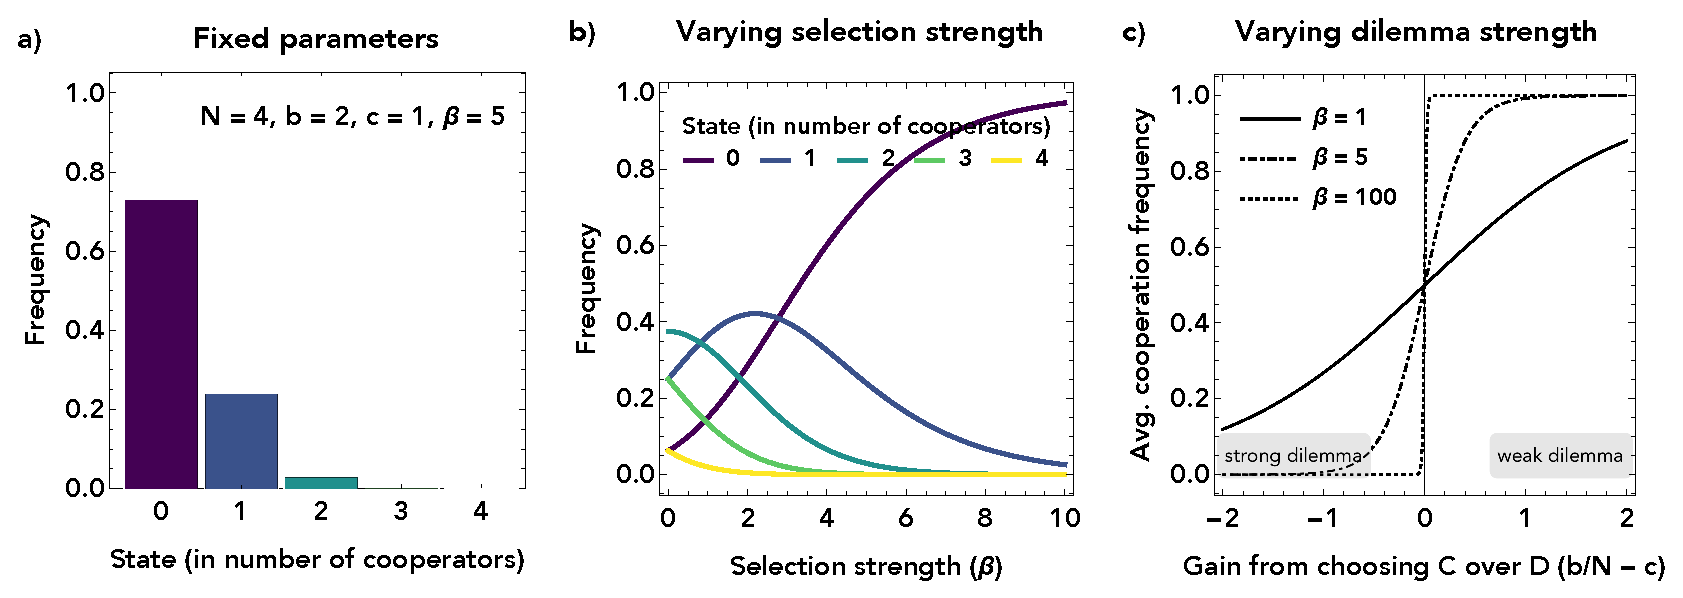
\includegraphics[width =  \textwidth]{figures/figure1.eps}~\\[0.4cm]
\caption{\onehalfspacing
\textbf{Symmetric linear public goods game.}
We use the following parameters for all the panels in this figure: $N = 4$ (group size), $b = 2$ (benefit provided to the public good on cooperation), $c = 1$ (cost of cooperation) a) Here we show the frequency of each state in the stationary distribution of introspection dynamics. As players are identical here, each state can be defined by the number of cooperators. We use a selection strength of $\beta = 5$ for the introspection dynamics. For this strength of selection, states with more cooperators are less likely than states with less cooperators in the stationary distribution b) The frequency of each state for varying selection strength, $\beta$. We use the same color code as the previous panel. Comparing neutrality ($\beta = 0$) with low to intermediate $\beta$ values, we see that selection favors states other than 0 cooperators. Indeed, up to $\beta \approx 3$, state $0$ is not the most frequent state in the long run c) Average cooperation frequency for varying dilemma strength depends on the selection strength $\beta$ and the parameters of the linear public goods game: $b,c, N$. We use the marginal gain of choosing cooperation over defection, $b/N - c$, as a measure of the dilemma strength. When this quantity is negative and low, we say that the dilemma is strong. In this case, there is no individual advantage to cooperate. When this quantity is positive and high, we say that the dilemma is weak. In this case, cooperation dominates defection. Typically, a linear public goods dilemma is defined to have a negative marginal gain (see conditions above). Here, we show the dilemma strength varying from $-2$ to $2$. The results are shown for different values of selection strength, $\beta = 1, 5$ and $100$. For high $\beta$, stationary distribution of the introspection dynamics reflects the rational play. In the long run player play the Nash equilibrium. When marginal gain is negative, defection is played with almost certainty (and \emph{vice-versa}). For low $\beta$, however, we see that some cooperation is possible even when the dilemma is strong. }
\label{Fig:LPGG-symmetric}
\end{figure}
\clearpage
\begin{figure}
\centering
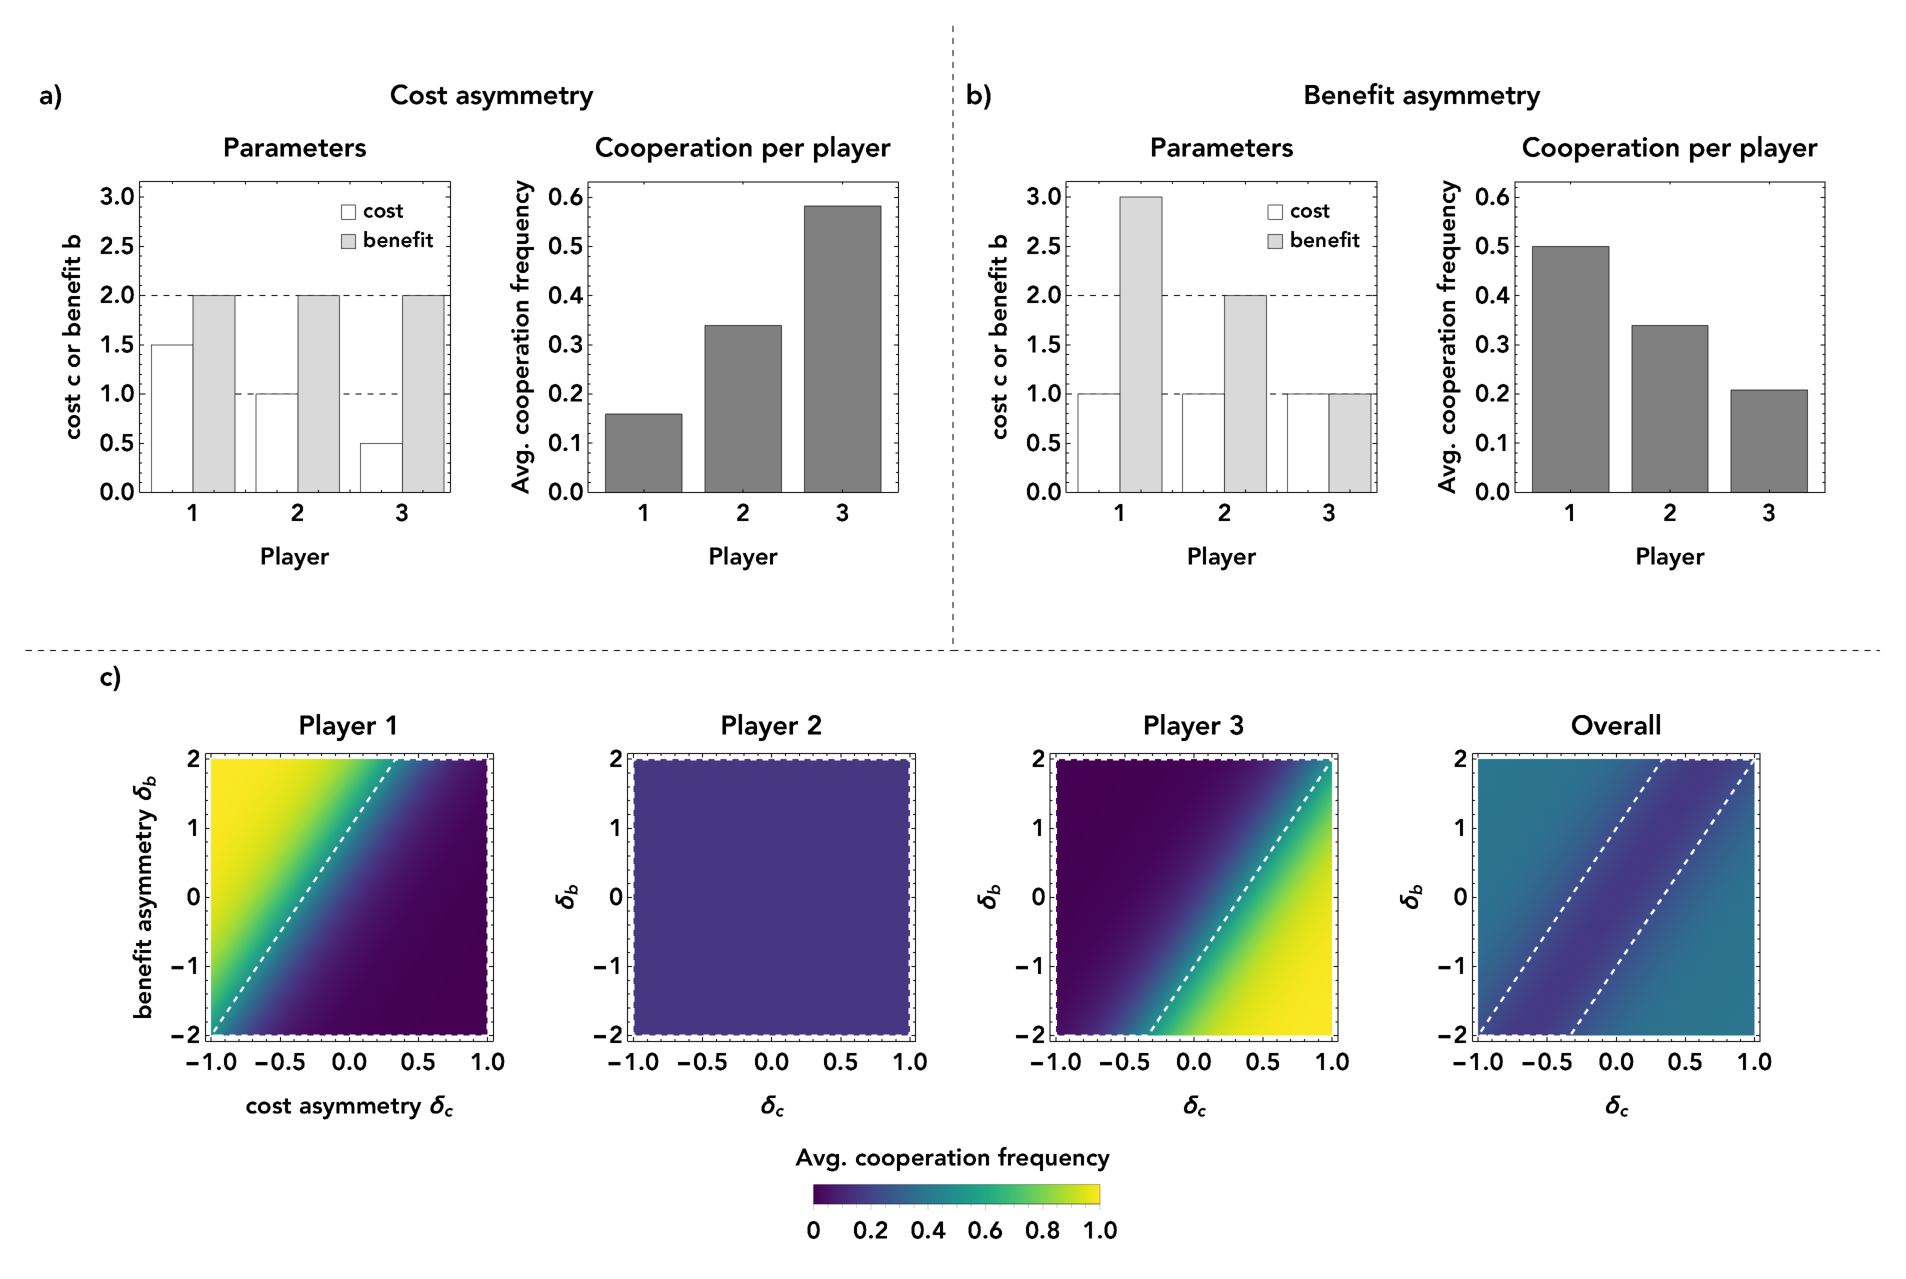
\includegraphics[width =  \textwidth]{figures/figure2.eps}~\\[0.4cm]
\caption{\onehalfspacing
\textbf{Asymmetric linear public goods game.} In the upper panels (a and b) we show the cost of cooperation and the benefit of provided due to cooperation for the three players on the left and the average cooperation frequency on the right. In this example, the cost of cooperation for players 1, 2 and 3 are $1 + \delta_c, 1$ and $1 - \delta_c$ respectively. The benefits that player 1, 2 and 3 provide upon cooperation are $2 + \delta_b, 2$ and $2 - \delta_b$ respectively. The cost and benefit for the reference player (player 2) are shown with black dashed lines in the left panels of a and b. In a) player 1 and 3 differ by 0.5 units in their cost of cooperation from the reference player. All the players provide the same benefit when they contribute (i.e., $\delta_b = 0$). Conversely, in b) benefit by player 1 and 3 differ from the reference player by 1 unit. The cost of cooperation is the same for all players ($c = 1$). In c), we vary the asymmetry strengths $\delta_c $ and $\delta_b$ simultaneously and show both average individual cooperation frequency and the overall average cooperation frequency in the long-run. The reference player's cost and benefit are 1 and 2 units respectively. The area within the white dashed lines represents the parameter values for which the marginal gain of choosing cooperation over defection is negative, for each single player and, in the right-most panel, for all players simultaneously. For panels a and b we use a selection strength of $\beta = 2$ while for panel c, we use a selection strength of $\beta = 5$. 
}
\label{Fig:LPGG-asymmetric}
\end{figure}
\clearpage
\begin{figure}
\centering
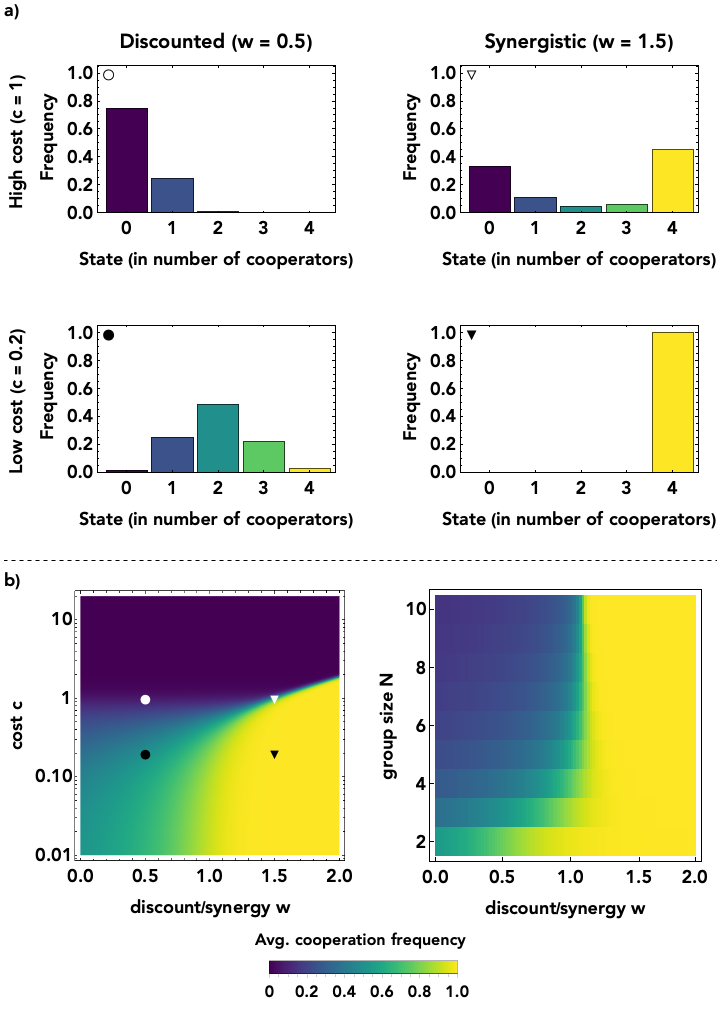
\includegraphics[width =  0.65\textwidth, keepaspectratio]{figures/figure3}~\\[0.4cm]
\caption{\onehalfspacing
\textbf{Symmetric general public goods game}. We study introspection dynamics in the general public goods game with 4 symmetric players, each having two possible actions - cooperation and defection. For a detailed description of the game, please see the main text. a) The frequency of each state in the stationary distribution of introspection dynamics in four types of multiplayer social dilemmas display qualitatively different results. The upper panels refer to a high cost of cooperation ($c=1$) while the bottom panels to a low cost of cooperation ($c = 0.2$); left panels refer to a discounted public good ($w = 0.5$), and the right panels refer to a synergistic public good ($w = 1.5$). Each case is tagged with a symbol that places the particular case in the contour plot in panel b, b) Average cooperation frequency for varying discount/synergy factor, $w$, and varying cost of cooperation, $c$. Cooperation is feasible when costs are not restrictively high and the public good is not too discounted. c) Average cooperation frequency for varying discount/synergy factor, $w$, and group size $N$. For this plot,the cost of cooperation for each player is $c = 0.4$. The feasibility of cooperation drops with larger group sizes when the public good is discounted. For all panels, the benefit of cooperation generated by each player is worth 2 units. The selection strength of the process is $\beta = 5$ for all panels.} 
\label{Fig:GPGG-symmetric}
\end{figure}
\clearpage
\begin{figure}
\centering
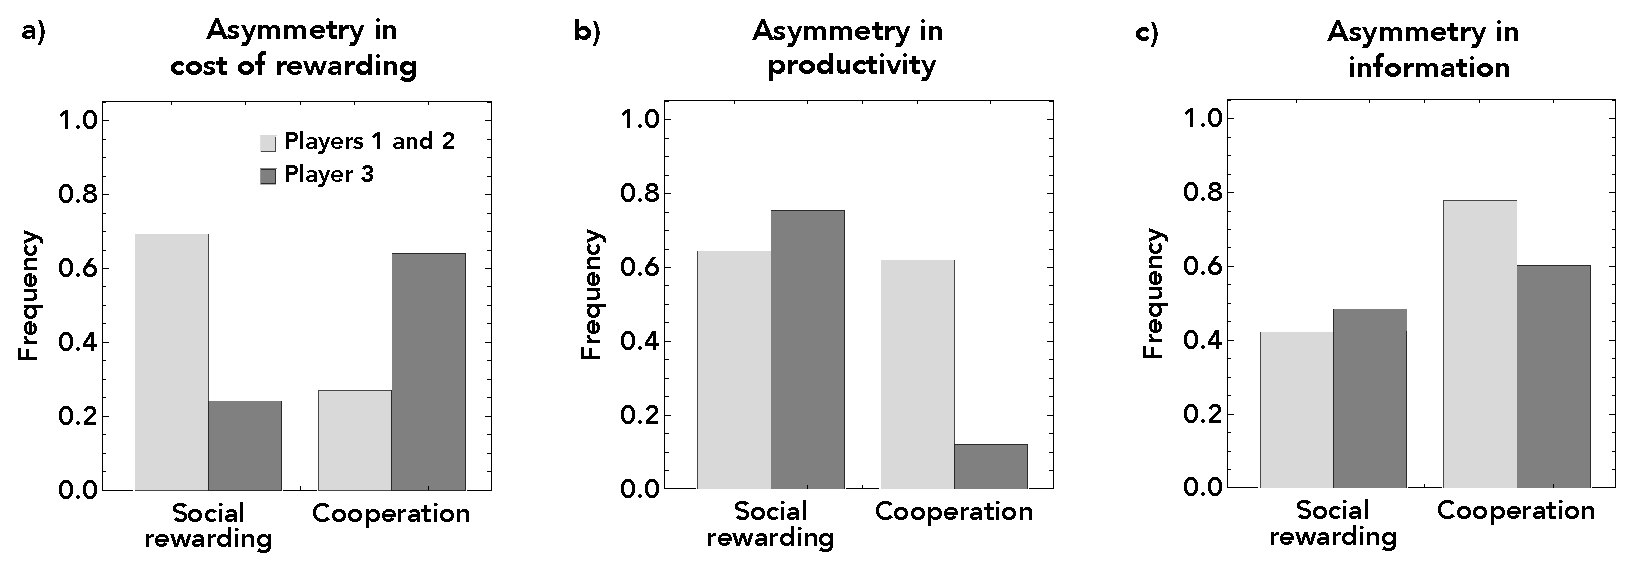
\includegraphics[width =  \textwidth]{figures/figure4.eps}~\\[0.4cm]
\caption{\onehalfspacing
\textbf{Cooperation and social rewarding in the stationary distribution of introspection dynamics in the linear public goods game with peer rewarding} Here we study a game with three asymmetric players, each having 16 possible strategies. Players cooperate in a linear public goods and then reward each other in the next stage after everyone's contribution is revealed. Players can condition their cooperation on the information they have about their co-players' rewarding strategies. For a full description of the model, please see the section on rewarding above. In this example, players 1 and 2 are identical in all aspects while player 3 is asymmetric to them in only a single aspect. In here, we plot the average frequency with which players cooperate and reward cooperation after a long time (after $10^5$ time steps of a computer simulation). We consider three types of asymmetry for player 3. a) First, we consider the case where player 3 has a high cost of rewarding compared to player 1 and 2, $0.7 = \gamma_3 > \gamma_1 = 0.1$. b) Then, we consider the case where player 3 is less productive than their co-players, $1.2 = r_3 < r_1 = 2$. c) Finally, we consider the case where player 3 has less information about co-players' rewarding strategies than their peers, that is, $0.1 = \lambda_3 < \lambda_1 = 0.9$. For all plots, we consider the selection strength of players are high, $\beta = 10$. Unless otherwise mentioned, the following parameters are maintained for all panels: $c_i = 1$ (individual cost of cooperation), $r_i = 2$ (individual productivity), $\gamma_i = 0.1$ (individual cost of cooperation), $\lambda_i = 0.9$ (individual information about co-players' strategies). In panels a and b, the reward value $\rho$ is 0.3 while for the last panel, c, the reward value $\rho = 1$.}
\label{Fig:SocialRewarding}
\end{figure}
\bibliographystyle{unsrt}
\clearpage

\newpage
\bibliography{bibtex}
\end{document}